\documentclass[10pt]{report}
\usepackage[utf8]{inputenc}
\usepackage[italian]{babel}
\usepackage{multicol}
\usepackage[bookmarks]{hyperref}
\usepackage[a4paper, total={18cm, 25cm}]{geometry}
\usepackage{graphicx}
\usepackage{xcolor}
\usepackage{textcomp}
\graphicspath{ {./img/} }
\usepackage{listings}
\usepackage{makecell}
\usepackage{qtree}
\usepackage{pgfplots}
\usepackage{tikz}
\usepgflibrary{shapes}
\usepgfplotslibrary{fillbetween}
\definecolor{backcolour}{RGB}{255,255,255}
\definecolor{codegreen}{RGB}{27,168,11}
\definecolor{codeblue}{RGB}{35,35,205}
\definecolor{codegray}{RGB}{128,128,128}
\definecolor{codepurple}{RGB}{205,35,56}
\lstdefinestyle{myPython}{
	backgroundcolor=\color{backcolour},   
	commentstyle=\color{codegreen},
	keywordstyle=\color{codeblue},
	numberstyle=\tiny\color{codegray},
	stringstyle=\color{codepurple},
	basicstyle=\small\ttfamily,
	breakatwhitespace=false,         
	breaklines=true,                 
	captionpos=b,                    
	keepspaces=true,                 
	numbers=left,                    
	numbersep=2pt,                  
	showspaces=false,                
	showstringspaces=false,
	showtabs=false,                  
	tabsize=2,
	language=python
}
\newcommand*\triangled[1]{\tikz[baseline=(char.base)]{
            \node[regular polygon, regular polygon sides=3,draw,inner sep=1pt] (char) {#1};}}
            
\usepackage{fancyhdr}
\pagestyle{fancy}
\renewcommand{\headrulewidth}{0pt}
\fancyhead{}
\fancyfoot[L]{Telegram: \texttt{@fexed}}
\fancyfoot[R]{Github: \texttt{fexed}}
\begin{document}
\title{Human Language Technologies}
\author{Federico Matteoni}
\date{A.A. 2021/22}
\renewcommand*\contentsname{Index}

\maketitle
\tableofcontents
\pagebreak
\section{Introduction}
Prof. Giuseppe Attardi\\
Prerequisites are: proficiency in Python, basic probability and statistics, calculus and linear algebra and notions of machine learning.
\paragraph{What will we learn} Understanding of and ability to use effective modern methods for \textbf{Natural Language Processing}. From traditional methods to current advanced ones like RNN, Attentions\ldots\\
Understanding the difficulties in dealing with NL and the capabilities of current technologies, with experience with \textbf{modern tools} and aiming towards the ability to build systems for some major NLP tasks: word similarities, parsing, machine translation, entity recognition, question answering, sentiment analysis, dialogue system\ldots
\paragraph{Books} Speech and Language Processing (Jurafsky, Martin), Deep Learning (Goodfellow, Bengio, Courville), Natural Language Processing in Python (Bird, Klein, Loper)
\paragraph{Exam} Project (alone or team of 2-3 people) with the aim to experiment with techniques in a realistic setting using data from competitions (Kaggle, CoNLL, SemEval, Evalita\ldots). The topic will be proposed by the team or chosen from a list of suggestions.
\paragraph{Experimental Approach}\begin{enumerate}
	\item Formulate hypothesis
	\item Implement technique
	\item Train and test
	\item Apply evaluation metric
	\item If not improved:\begin{list}{}{}
		\item Perform error analysis
		\item Revise hypothesis
	\end{list}
	\item Repeat!
\end{enumerate}
\paragraph{Motivations} Language is the most distinctive feature of human intelligence, \textbf{it shapes thought}. Emulating language capabilities is a scientific challenge, a \textbf{keystone for intelligent systems} (see: Turing test)
\paragraph{Structured vs unstructured data} The largest amount of information shared with each other is unstructured, primarily text. Information is mostly communicated by e-mails, reports, articles, conversations, media\ldots and attempts to turn text to structured (HTML) or microformat only scratched the surface.\\
Problems: requires universal agreed \textbf{ontologies} and additional effort. Entity linking attempts to provide a bridge.
\section{State of the Art}
\paragraph{Early History} During 1950s, up until AI winter.
\paragraph{Resurgence in the 1990s} Thanks to statistical methods, novelty, to study language. Challenges arise: NIST, Netflix, DARPA Grand Challenge\ldots\\
During 2010s: deep learning, neural machine translation\ldots
\paragraph{Statistical Machine Learning} Supervised training with \textbf{annotated} documents.\\
The paradigm is composed of the following:
\begin{list}{}{}
	\item Training set $\{x_i,y_y\}$
	\item Representation: choose a set of features to represent data $x\mapsto \phi(x) \in R^D$
	\item Model: choose an hypothesis function to compute $f(x) = F_\Theta(\phi(x))$
	\item Evaluation: define the cost function on error with respect to examples $J(\Theta) = \sum_i (f(x_i) - y_i)^2$
	\item Optimization: find parameters $\Theta$ that minimize $J(\Theta)$
\end{list}
It's a generic method, applicable to any problem.
\paragraph{Traditional Supervised Learning Approach} Freed us from devising algorithms and rules, requiring the creation of annotated training sets and imposing the tyranny of feature engineering.\\
Standard approach for each new problem:
\begin{list}{}{}
	\item Gather as much labeled data as one can
	\item Throw a bunch of models at it
	\item Pick the best
	\item Spend hours hand engineering some features or doing feature selection/dimensionality reduction
	\item Rinse and repeat
\end{list}
\paragraph{Technological Breakthroughs} Improved ML techniques but also large annotated datasets and more computing power, provided by GPUs and dedicated ML processors (like the TPU by Google).\\
ML exploits parallelism: stochastic gradient descent can be parallelized (asynchronous stochastic gradient descent). No need to protect shared memory access, and low (half, single) precision is enough.
\paragraph{Deep Learning Approach} Was a big breakthrough.\begin{list}{}{}
	\item Design a model architecture
	\item Define a loss function
	\item Run the network letting the parameters and the data representations \textbf{self-organize} as to minimize the loss
	\item End-to-end learning: no intermediate stages nor representation
\end{list}
\subparagraph{Feature representation} Use a vector with each entry representing a feature of the domain element\\
	Deep Learning represents data as vectors. Images are vectors (matrices), but words? \textbf{Word Embeddings}: transform a word into a vector of hundreds of dimensions capturing many subtle aspects of its meaning. Computed by the means of \textbf{language model}.\\
From a discrete to distributed representation. Words meaning are dense vectors of weights in a high dimensional space, with algebraic properties.\\
Background: philosophy, linguistics and statistics ML (feature vectors).
\subparagraph{Language Model} Statistical model which tells the probability that a word comes after a given word in a sentence.
\subparagraph{Dealing with Sentences} A sentence is a sequence of words: build a representation of a sequence from those of its words (compositional hypothesis). Sequence to sequence models.\\
Is there more structure in a sentence than a sequence of words? In many cases, tools forgets information when translating sentences into sequences of words, discarding much of the structure.
\section{Language Modeling}
\paragraph{Probabilistic Language Model} The goal is to assign a probability to a sentence.
\begin{list}{}{}
	\item \textbf{Machine Translation}: $P($high winds tonight$) > P($large winds tonight$)$
	\item \textbf{Spell Correction}: $P($about fifteen minutes from$) > P($about fifteen minuets from$)$
	\item \textbf{Speech Recognition}: $P($I saw a van$) > P($eye saw a van$)$
	\item \textbf{Language Identification}: $s$ from unknown language (italian or english) and $L$ita, $L$eng language models for italian and english $\Rightarrow$ $L$ita$(s) > L$eng$(s)$
	\item Summarization, question answering\ldots
\end{list}
We want to compute \begin{list}{}{}
	\item $P(W) = P(w_1,w_2,\ldots,w_n)$ the probability of a sequence
	\item $P(w_4\:|\:w_1,w_2,w_3,w_4)$ the probability of a word given some previous words
\end{list}
The model that computes that is called the \textbf{language model}
\paragraph{Markov Model and N-Grams} Simplify the assumption: the probability of a word given all the previous is the same of the probability of that word given just few (one, two\ldots) previous words. So $P(w_i\:|\:w_{i-},\ldots,w_1) = P(w_i\:|\:w_{i-1})$ (First order Markov chain).\\
With a \textbf{$N$-gram}: $P(w_n\:|\:w_1^{n-1}) \simeq P(w_n\:|\:w_{n-N+1}^{n-1})$\\
In general it's insufficient: language has \textbf{long distance dependencies}, but we can often get away with $N$-gram models. For example:\begin{list}{}{}
	\item “The \textbf{man} next to the large oak tree near the grocery store on the corner \textbf{is} tall.”
	\item “The \textbf{men} next to the large oak tree near the grocery store on the corner \textbf{are} tall.”
\end{list}
Or even semantic dependencies:
\begin{list}{}{}
	\item “The \textbf{bird} next to the large oak tree near the grocery store on the corner \textbf{flies} rapidly.”
	\item “The \textbf{man} next to the large oak tree near the grocery store on the corner \textbf{talks} rapidly.”
\end{list}
So more complex models are needed to handle such dependencies.
\paragraph{Maximum likelihood estimate}$$P(w_n\:|\:w_{n-N+1}^{n-1}) = \frac{\hbox{count}(w_{n-N+1}^{n-1},w_n)}{\hbox{count}(w_{n-N+1}^{n-1})}$$
Maximum because it's the one that maximize $P($Training set $|$ Model$)$
\paragraph{Shannon Visualization Method} Generate random sentences:
\begin{list}{}{}
	\item Choose a random bigram $(\langle s\rangle,w)$ according to its probability
	\item Choose a random bigram $(w,x)$ according to its probability
	\item Repeat until we pick $\langle/s\rangle$
\end{list}
\paragraph{Shannon Game} Generate random sentences by selecting the words according to the probabilities of the language models.
\begin{lstlisting}[style=myPython]
def gentext(cpd, word, length=20):
	print(word, end = ' ')
	for i in range(length):
		word = cpd[word].generate()
		print(word, end = ' ')
	print("")
\end{lstlisting}
\paragraph{Perils of Overfitting} N-grams only word well for word prediction if the test corpus looks like the training corpus. In real life, this is often not the case.\\
We need to train robust models able to adapt.
\subparagraph{Smoothing} Many rare (but not impossible) combinations of word sequences never occur in training, so MLE incorrectly assigns zero to many parameters (sparse data).\\
If a new combination occurs during testing, it is given a probability of zero and the entire sequence gets a probability of zero (infinite perplexity).\\
Parameters are \textbf{smoothed}/regularized to reassign some probability mass to unseen events (meaning removing probability from seen ones in order to maintain the joint distribution that sums to 1)
\paragraph{Zipf's Law} A small number of events occur with high frequency, while a large number of events occur with small frequency. You can quickly collect statistics on the high frequency events, but you may have to wait an arbitrarily long time to get valid statistics on low frequency events.\\
The result is that our estimates are sparse. No counts at all for the vast bulk of things we want to estimate. Some of the zeroes in the table are really zeroes, but others are simply low frequency events you haven't seen yet: after all, anything can happen. How to address? By estimating the likelihood of unseen N-grams.
\begin{center}
	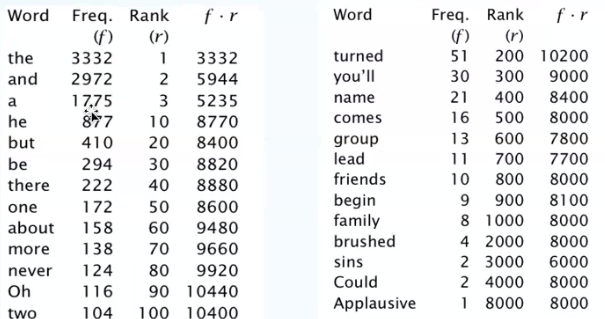
\includegraphics[scale=0.75]{1.png}
\end{center}
\textbf{Result}: $f$ is proportional to $\frac{1}{r}$, meaning that there is a constant $k\:|\:f\cdot r = k$
\begin{center}
	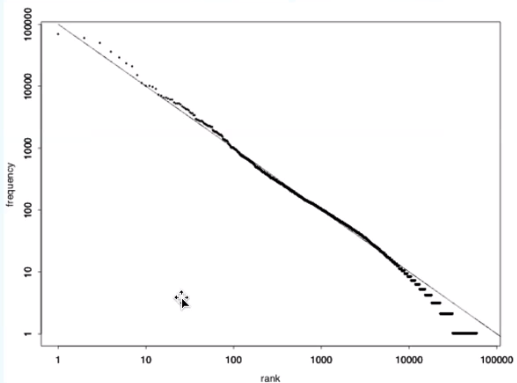
\includegraphics[scale=0.75]{2.png}
\end{center}
\subsection{Evaluation and Perplexity}
\paragraph{Evaluation} Train parameters of our model on a training set. For the evaluation, we apply the model on new data and look at the model's performance: \textbf{test set}. We need a metric which tells us how well the model is performing: one of such is \textbf{perplexity}.
\paragraph{Extrinsic Evaluation} Evaluating N-gram models.\begin{list}{}{}
	\item Put model A in a task (language identification, speech recognizer, machine translation system\ldots)
	\item Run the task, get an accuracy for $A$
	\item Put model B in the task, get accuracy for B
	\item Compare the accuracies
\end{list}
\paragraph{Language Identification Task} Build a model for each language and compute probability that text is of such language.
$$lang = arg\max_l P_l(text)$$
\paragraph{Difficulty of Extrinsic Evaluation} Extrinsic evaluation is time-consuming, can take days to run an experiment. Recent benchmarks like GLUE have become popular due to the effectiveness.\\
Intrinsic evaluation us an approximation called \textbf{perplexity}: it's a poor approximation unless the test data looks just like the training data.
\paragraph{Perplexity} The intuition is the notion of surprise: how surprised is the language model when it sees the test set? Where surprise is a measure of "I didn't see that coming". The more surprised is, the lower the probability it assigned to the test set, and the higher the probability the less surprised it is.\\
So perplexity measures how well a model "fits" the test data. It uses the probability that the model assigns to the test corpus and normalizes for the number of words in the test corpus, taking the inverse. $$PP(w) = \sqrt[N]{\frac{1}{P(w_1\ldots w_N)}}$$
Measures the weighted average branching factor in predicting the next word (lower is better).\\
In the chain rule $$PP(w) = \sqrt[N]{\prod_{i=1}^N\frac{1}{P(w_i\:|\:w_1\ldots w_{i-1})}}$$
And for bigrams $$PP(w) = \sqrt[N]{\prod_{i=1}^N\frac{1}{P(w_i\:|\:w_{i-1})}}$$
Lower perplexity $\Rightarrow$ better model
\section{Representation of Words}
\paragraph{Word Meaning} Definition of \textbf{meaning}:\begin{list}{}{}
	\item Idea represented by a word, phrase\ldots
	\item Idea that a person wants to express by using words, signs\ldots
	\item Idea expressed in a work of writing, art\ldots
\end{list}
\textbf{Signifier} (symbol) $\Leftrightarrow$ \textbf{Signified} (idea or concept) = \textbf{denotation}
\paragraph{Linguistic Solution} Dictionary or lexical resources provide word definitions as well as synonyms, hypernums, antonyms\ldots example: \textbf{Wordnet}.
\subparagraph{Problems with lexical resources} \begin{list}{}{}
	\item Imperfect, sometimes there are errors
	\item Missing new meanings of words, hard to keep up-to-date
	\item Subjective
	\item Require human labor to create and adapt
	\item Hard to compute accurate word similarity
\end{list}
\paragraph{Vector Space Model} The \textbf{VSM} is a representation for text used in information retrieval. A document is represented by a vector in a $n$-dimensional space $$v(d_1) = [t_1,\ldots, t_n]$$
Each dimension corresponds to a separate term.\\
The VSM considers words as discrete symbols.
\subparagraph{One Hot Representation} A word occurrence is represented by one-hot vectors, with the vector dimension being the number of words in a vocabulary and $1$ in correspondence of the position of the represented word. Useful for representing a document by the sum of the word occurrence vector, and document similarity given by \textbf{cosine distance} (angle between vectors).
\subparagraph{tf*idf Measure} Term frequency: frequency of the word.\\
Inverse document frequency (idf): given $N$ total documents and $df_i=$ document frequency of word $i$, meaning the number of documents with word $i$
$$idf_i=\log\frac{N}{df_i}$$
\subparagraph{Classical VSM} Vector is all zeroes with $idf_t$ instead of $1$. The vector of a document is the sum of the vectors of its terms occurrence vectors.\\
Doesn't capture similarity between terms.
\paragraph{Problems with Discrete Symbols} All vectors are orthogonal, with no notion of similarity. Search engines try to address the issue using WordNet synonyms but it's better to encode the similarity in the vectors themselves.
\subparagraph{Intuition} Model the meaning of a word by "embedding" it in a vector space. The meaning of a word is a vectors of numbers (vector models are also called \textbf{embeddings}), so a \textbf{dense vector space}. Contrast: word meaning is represented in many computational linguistic applications by a vocabulary index.
\paragraph{Word Vectors/Embeddings} Build dense vector for each word chosen so that it is similar to vectors of words that appear in similar contexts.\\
Four kinds:\begin{enumerate}
	\item[] Sparse Vector Representations
	\item Mutual-information weighted word co-occurence matrices
	\item[] Dense Vector Representations
	\item Singular Value Decomposition (and Latent Semantic Analysis)
	\item Neural Network Inspired models (word2vec, GloVe, fastText\ldots)
	\item Brown Clusters
\end{enumerate}
\paragraph{Distributional Hypothesis} A word's meaning is given by the words that frequently appear close-by. Old idea but successful just with modern statistical NLP.\\
When a word $w$ appears in a text, its context is the set of words that appear nearby (within a fixed-size window). Use of the many contexts of $w$ to build a representation of $w$.
\subparagraph{Word Context Matrix} Is a $|V|\times|V|$ matrix $X$ that counts the frequencies of co-occurrence of words in a collection of contexts (i.e. text spans of a given length).
\subparagraph{Co-Occurrence Matrix} Words $\equiv$ Context words. Rows of $X$ capture similarity yet $X$ is still high dimensional and sparse. One row per word with counts of occurrencies of any other word.\\
We can compute the distance vectors between words, but neighboring words are not semantically related.
\subsection{Word Embeddings}
\paragraph{Dense Representations} Project word vectors $v(t)$ into a low dimensional space $R^k$ with $k<<|V|$ of continuous space word representations (a.k.a. \textbf{embeddings})
$$Embed : R^{|V|}\rightarrow R^k$$
$$Embed(v(t)) = e(t)$$
Desired properties: remaining dimensions represent the most salient features, so the words with syntactic/semantic similarities are grouped close in space.
\paragraph{Collobert} Build embeddings and estimate whether the word is in the proper context using a neural network. Positive examples from text, and negative examples made replacing center word with random one. The loss for the training is $$Loss(\Theta) = \sum_{x\in X}\sum_{w\in W} \max(0, 1-f_\Theta(x) + f_\Theta(x^{(w)}))$$
with $x^{(w)}$ obtained by replacing the central word of $x$ with a random word.
\paragraph{Word2Vec} Framework for learning words, much faster to train. Idea:\begin{list}{}{}
	\item Collect a large corpus of text
	\item Every word in a fixed vocabulary is represented by a vector
	\item Go through each position $t$ in the text, which has a center word $c$ and context ("outside") words $o$
	\item Use the similarity of the word vectors for $c$ and $o$ to calculate the probability of $o$ given $c$
	\item Keep adjusting word vectors to maximize this probability
\end{list}
Two kinds:
\begin{center}
	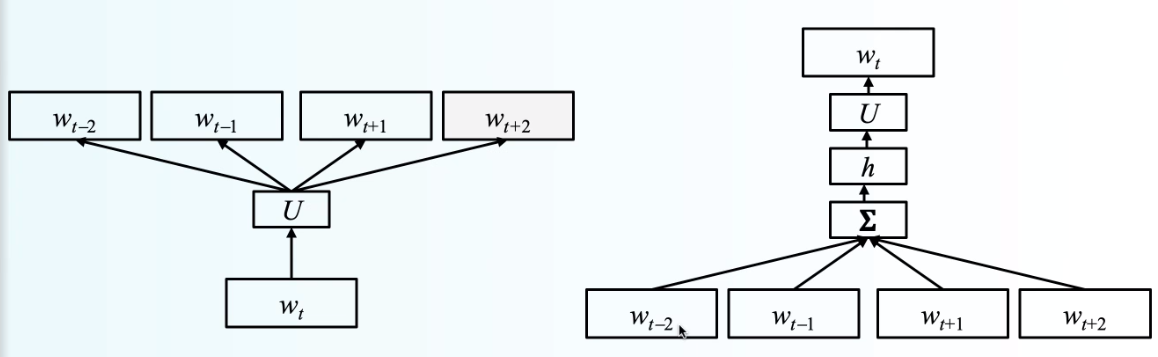
\includegraphics[scale=0.5]{3.png}
\end{center}
\begin{list}{}{}
	\item Skip-gram: predict context words within window of size $m$ given the center word $w_t$
	\begin{center}
		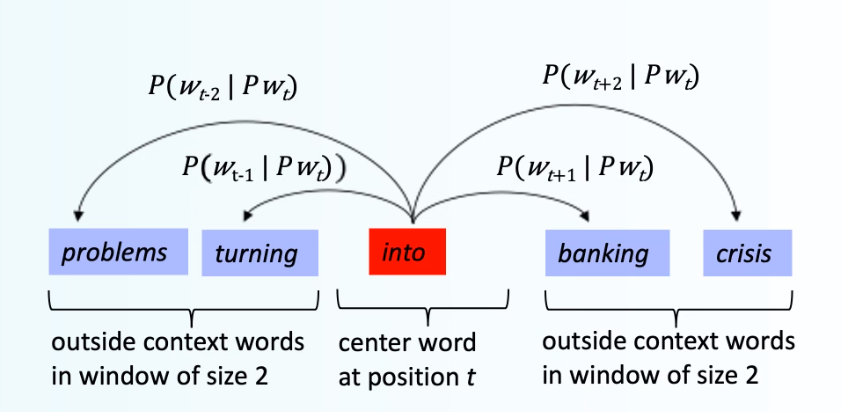
\includegraphics[scale=0.4]{4.png}
	\end{center}
	\item CBoW: predict center word $w_t$ given context words within window of size $m$
\end{list}
Embeddings are a by-product of the word prediction task. Even though it's a prediction task, the network can be trained on any text (no need for human-labeled data!).\\
Usual context size is 5 words before and after. Features can be multi-word expressions. Longer windows can capture more semantics and less syntax.\\
A typical size for $h$ is 200-300.
\subparagraph{Skip-Gram}
\begin{multicols}{2}
\begin{list}{}{}
	\item Inputs are one-hot representation of the word
	\item $w\in R^{|Vocabulary|}$ are high-dimensional
	\item $v\in R^d$ is low dimensional: size of the embedding space $d$
	\item $V\in R^{|Voc|\times d}$ input word matrix
	\item row $t$ of $V$ is the input vector, representation for \textbf{center} word $w_t$
	\item $U\in R^{d\times|Voc|}$ output matrix
	\item column $o$ of $U$ is the output vector, representation for \textbf{context} word $w_o$
\end{list}
\columnbreak
\begin{center}
	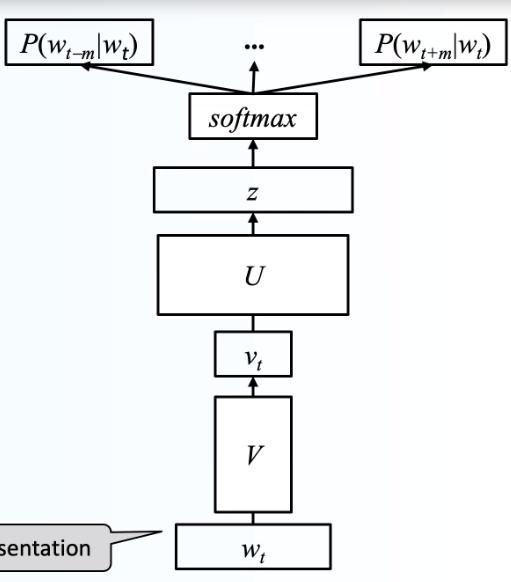
\includegraphics[scale=0.35]{5.png}
\end{center}
\end{multicols}
$v_t = w_tV$ embedding of word $w_t$\\$z=v_tU$ $z_i$ is the similarity of $w_t$ with $w_i$\\Softmax converts $z$ to a probability distribution $p_i$ $$p_i=\frac{e^{z_i}}{\sum_{j\in V}e^{z_j}}$$
Procedure
\begin{list}{}{}
	\item Lookup the embedded word vector for the center word $v_c = V[c] \in R^n$
	\item Generate score vector $z = v_cU$
	\item Turn the score vector into probabilities $\hat{y} =$ softmax$(z)$
\end{list}
$\hat{y}_{c-m},\ldots$ Those are the estimates of the probabilities of observing each context word. These should match the true probabilities, which are $$y^{c-m},\ldots, y^{(c-1)}, y^{(c+1)}, \ldots, y^{(c+m)}$$
The training iterates through the whole corpus predicting surrounding words given the center word.
\subparagraph{Objective Function} For each position $t=1,\ldots,T$ predict context words within a windows of fixed size $m$ given each center word $w_t$ $$\hbox{Likelihood} = L(\Theta) = \prod_{t=1}^T\prod_{-m\leq j\leq m,\:\:j\neq 0} P(w_{t+j}\:|\:w_t,\Theta)$$
While the objective function $J(\Theta)$ is the average negative log likelihood $$J(\Theta) = -\frac{1}{T}\log L(\Theta) = -\frac{1}{T}\sum_{t=1}^T\sum_{-m\leq j\leq m,\:\:j\neq 0} \log(P(w_{t+j}\:|\:w_t,\Theta)=$$
To compute $P(o\:|\:c, \Theta)$ we use two vectors per word $w$: $v_w$ when $w$ center word and $u_w$ when $w$ context word. For a center word $c$ and a context word $o$:$$P(o\:|\:c) = \frac{e^{u_o v_c}}{\sum_{w\in V} e^{u_w v_c}}$$
With the dot product $u\cdot v = \sum_i u_iv_i$: larger product $\Rightarrow$ larger probability. Normalize over entire vocabulary to give probability distribution.\\
$J(\Theta)$ is a function of all windows in the corpus, potentially billions: too expensive to compute. The solution is the stochastic gradient descent, sampling windows randomly and update after each one.
\paragraph{Softmax}\begin{list}{}{}
	\item Soft because still assign some probability to smaller $x_i$
	\item Max because amplifies the probability of largest $x_i$
\end{list}
\paragraph{Can we really capture the concept represented by a word?} Philosophical debate.
\paragraph{Negative Sampling} $\log\sum_{j\in F}e^{u_j}$ has lots of terms, costly to compute. The solution is to compute it only on a small sample of negative samples, i.e. $\log\sum_{j\in E}e^{u_j}$ where words $E$ are a few (e.g. 5) and sampled using a biased unigram distribution $U$ computed on training data
$$P(w) = \frac{U(w)^{\frac{3}{4}}}{\sum_{w_j\in V}U(w_j)^{\frac{3}{4}}}$$
\paragraph{CBoW} Continuous Bag of Words\\
Mirror of the skip-gram, where context words are used to predict target words.\\
$h$ is computed from the average of the embeddings of the input context, $z_i$ is the similarity of $h$ with the words embedding of $w_i$ from $U$.
\paragraph{Which Embeddings} $V$ and $U$ both define embeddigns, which to use? Usually just $V$. Sometimes average pairs of vectors from $V$ and $U$ into a single one or append one embedding vector after the other, doubling the length.
\paragraph{GloVe} Global Vectors for Word Representation. Insight: the ratio of conditional probabilities may capture meaning.
$$J = \sum_{i,j=1}^V f(X_{ij})\ldots$$
\paragraph{fastText} Similar to CBoW, word embeddings averaged to obtain good sentence representation. Pretrained models.
\paragraph{Co-Occurrence Counts}
$$P(w_t,w_{t-i},\ldots,w_{t-1}) = \frac{P(w_t,w_{t-i},\ldots,w_{t-1})}{P(w_{t-i},\ldots,w_{t-1})}$$
It's a big matrix, of $|V|\times|V|\simeq 100$k$\times100$k $\Rightarrow$ dimensionality reduction: principal component analysis, Hellinger PCA, SVD\ldots trying to reduce to size to $100$k$\times 50$, $100$k$\times 100$ or something similar, assigning each word a vector of $50$, $100$ or similar features.
\paragraph{Weighting} Weight the counts using corpus-level statistics to reflect co-occurrence significance: \textbf{Pointwise Mutual Information} $$ PMI(w_t,w_{t-i},\ldots,w_{t-1}) = \frac{P(w_t,w_{t-i},\ldots,w_{t-1})}{\log P(w_t)P(w_{t-i},\ldots,w_{t-1})} = \log\frac{\#(w_t,w_{t-i},\ldots,w_{t-1})\cdot|V|}{\#(w_{t-i},\ldots,w_{t-1})\#(w_t)}$$
Skip-gram model implicitly factorizes a shifted PMI matrix.\\
Idea of Singular Value Decomposition:
\begin{center}
	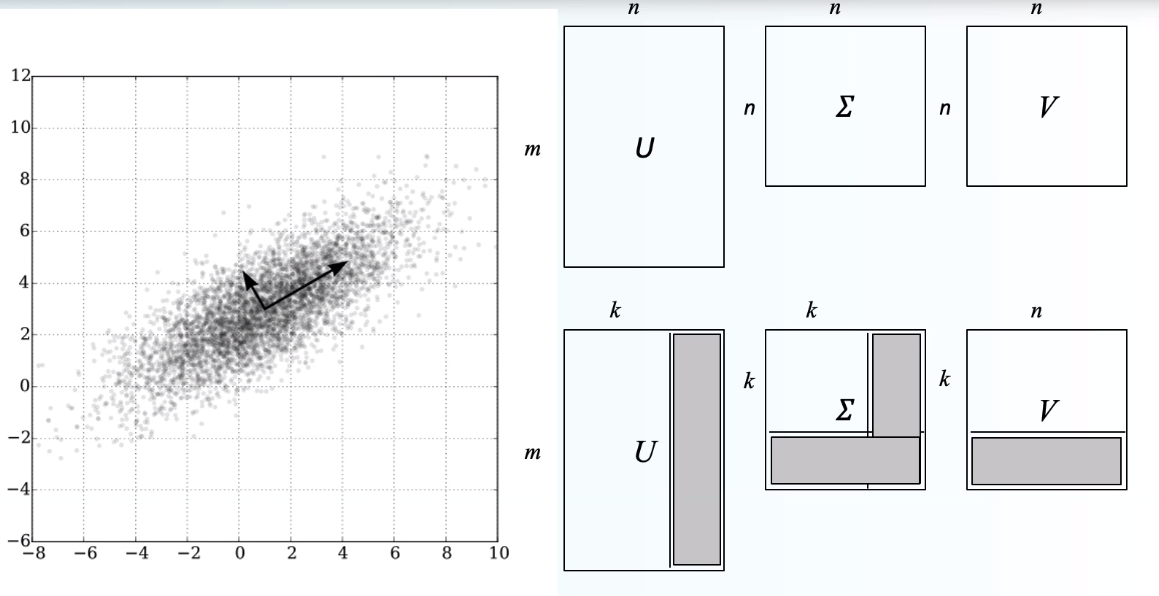
\includegraphics[scale=0.5]{6.png}
\end{center}
\subparagraph{Which One?} No clear winner. Parameters play a relevant role in the outcome of each method. Both SVD and SGNS performed well on most tasks, never underperforming significantly.\\
SGNS is suggested to be a good baseline: faster to compute and performs well.
\paragraph{Parallel word2vec} How to synchronize access to V and U, given multicore CPU to run SGD in parallel? No synchronization is good, because computation is stochastic hence it is approximate anyhow. Parameters are huge: low likelihood of concurrent access to the same memory cell. The effect is a very fast training.
\paragraph{Computing embeddings} The training cost of word2vec is linear in the size of the input. The training algorithm works well in parallel, given sparsity of words in contexts and use of negative sampling. It can be halted and restarted at anytime.
\paragraph{Gensim} Cython
\paragraph{Fang} Uses PyTorch
\subsection{Evaluation}
\paragraph{Polysemy} Word vector is a linear combination of its word senses.
$$v_{pike} = \alpha_1v_{pike_1} + \alpha_2v_{pike_3} + \alpha_3v_3$$
with $\alpha_i = \frac{f_i}{f_1+f_2+f_3}$ for the frequencies $f_i$.\\
It's intrinsic evaluation.
\paragraph{Extrinsic Vector Evaluation} The proof of the pudding is in the eating. Test on a task, e.g. NER (Named Entity Recognition)
\subsubsection{Embeddings in Neural Networks} An embedding layer is often used as fist layer in a neural network for processing text.\\
It consists of a matrix $W$ of size $|V|\times d$ where $d$ is the size of the embedding space. $W$ maps words to dense representations.\\
It is initialized either with random weights or pretrained embeddings. During learning, weights can be:
\begin{list}{}{}
	\item kept fixed (makes sense only when using pre-trained weights)
	\item updated, to adapt embeddings to the task
\end{list}
\begin{center}
	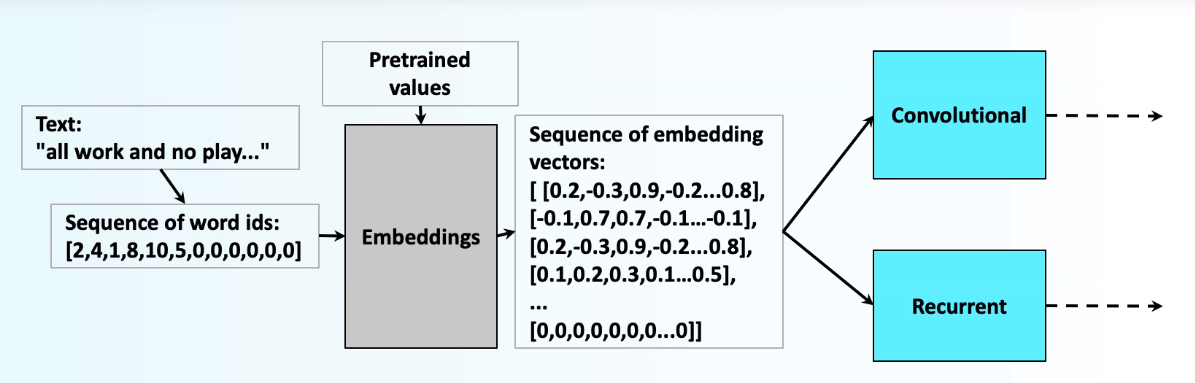
\includegraphics[scale=0.5]{7.png}
\end{center}
\subsubsection{Limits of Word Embeddings} \begin{list}{}{}
	\item Polysemous words
	\item Limited to words (neither multi words nor phrases)
	\item Represent similarity: antinomies often appear similar.\\
	Not good for sentiment analysis or polysemous words. Example:
	\begin{list}{}{}
		\item The movie was \textbf{exciting}
		\item The movie was \textbf{boring}
	\end{list}
\end{list}
\paragraph{Word Senses and Ambiguity}
\paragraph{Sentiment Specific}
\paragraph{Context Aware Word Embeddings}
\paragraph{ELMo} Embeddings from Language Model
\begin{center}
	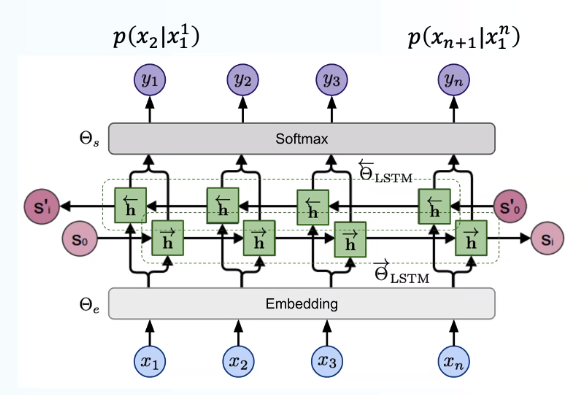
\includegraphics[scale=0.5]{8.png}
\end{center}
Given a sequence of $n$ tokens ($x_1,\ldots,x_n$), the language model learns to predict the probability of next token given the history
$$P(x_1,\ldots,x_n)=\prod_{i=1}^n P(x_i\:|\:x_1^{i-1})$$
The model is trained to minimize the negative log likelihood
$$L = -\sum_{i=1}^n\left(\log P(x_i\:|\:x_1^{i-1})+\log P(x_i\:|\:x_{i+1}^n) \right)$$
\paragraph{BERT} Semi-supervised training on large amounts of text, or supervised training on a specific task with a labeled dataset.
\section{Text Classification}
For example: positive/negative review identification, author identification, spam identification, subject identification\ldots
\paragraph{Definition} The classifier $f : D \rightarrow C$ with
\begin{list}{}{}
	\item $d\in D$ input document
	\item $C=\{c_1,\ldots,c_K\}$ set of classes
	\item $c\in C$ predicted class as output
\end{list}
The learner has
\begin{list}{}{}
	\item Input: a set of $N$ hand-labeled documents $T=\{(d_1,c_1),\ldots,(d_N,c_N)\}$
	\item Output: a learned classifier $f:D\rightarrow C$
\end{list}
\begin{center}
	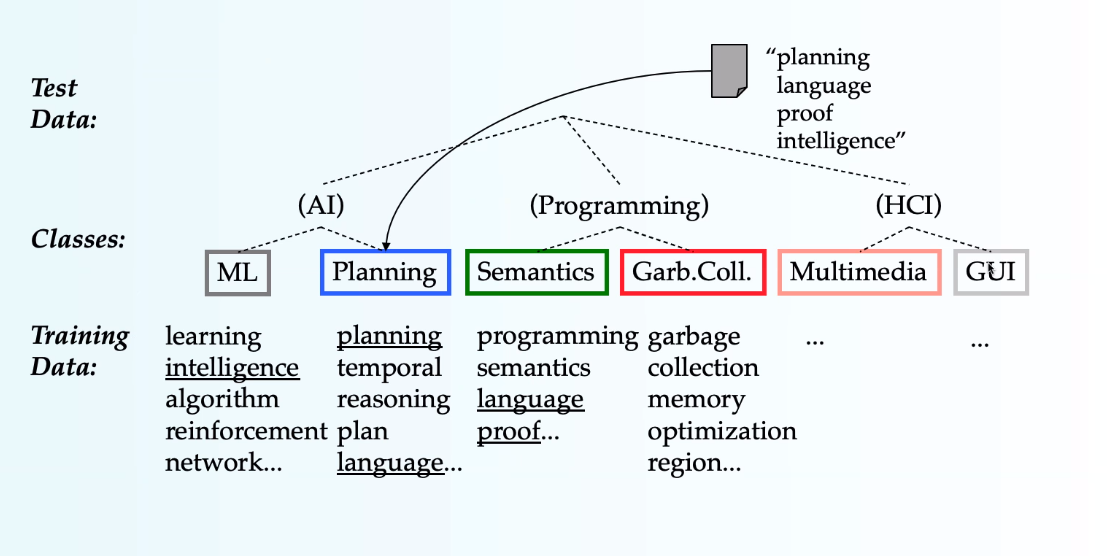
\includegraphics[scale=0.5]{9.png}
\end{center}
\paragraph{Hand-Coded Rules} Often very high accuracy, but building and maintaining these rules is expensive. For example: assign category if a document contains a given boolean combination of words (e.g. a blacklist of words for spam classification).
\paragraph{Supervised Machine Learning} Input \begin{list}{}{}
	\item A document $d\in D$
	\item A fixed set of classes $C=\{c_1,\ldots,c_K\}$
	\item A training set of $N$ hand-labeled documents $T=\{(d_1,c_1),\ldots,(d_N,c_N)\}$
\end{list}
As output\begin{list}{}{}
	\item A learned classifier $\gamma : D \rightarrow C$
\end{list}
\subsection{Naive Bayes}
A method based on the Bayes rule, relying on simple document representation (bag of words)
\paragraph{Bag of words representation} From a text, we count the frequency of each word.
\paragraph{Bayes Rule} Allows to swap the conditioning, useful because sometimes is easier estimating one kind of dependence than the other. $$P(B\:|\:A)=\frac{P(A\:|\:B)P(B)}{P(A)}$$
Applied to documents $d\in D$ and classes $c\in C$
$$P(c,d) = P(c\:|\:d)P(d) = P(d\:|\:c)P(c)$$
$$P(c\:|\:d) = \frac{P(d\:|\:c)P(c)}{P(d)}$$
\paragraph{Text classification problem} Using a supervised learning method, we want to learn a classifier $\gamma:X\rightarrow C$. The supervised learning method is denoted with $\Gamma(T)=\gamma$: it takes the training set $T$ as input and returns the learned classifier $\gamma$ that can be applied to the test set.
\subsubsection{Naive Bayes Classifiers}
We represent an instance $D$ based on some attributes $D=(x_1,\ldots, x_n)$\\Task: classify a new instance $D$ based on a tuple of attribute values into one of the calsses $c_j\in C$
$$C_{MAP}=\arg\max_{c_j\in C} P(x_1,\ldots,x_n\:|\:c_j)P(c_j)$$
\paragraph{Naive Bayes Assumption}
\begin{list}{}{}
	\item $P(c_j)$ can be estimated from the frequency of classes in the training examples
	\item $P(x_1,\ldots,x_n\:|\:c_j)$ has $O(|X|^n\cdot |C|)$ parameters and could only be estimated if a very very large number of training examples was available.
\end{list}
The \textbf{Naive Bayes Conditional Independence Assumption} is to assume that the probability of observating the conjunction of attributes is equal to the product of the individual probabilities $P(x_i\:|\:c_j)$. This means that features are independent of each other given the class
$$P(x_1,\ldots,x_n\:|\:c_j) = P(x_1\:|\:c_j)\cdot\ldots\cdot P(x_n\:|\:c_j)$$
\subsubsection{Multinomial Naive Bayes Text Classification}
$$C_B = \arg\max_{c_j\in C}P(c_j)\prod_i P(x_i\:|\:x_j)$$
Still too many possibilities. Assume the classification is independent of the position of the words, and use the same parameters for each position. The result is a \textbf{bag of words model} (over tokens, not types).
\paragraph{Learning the Model} Maximum likelihood estimate: simply use the frequencies in the data
$$\hat{P}(c_j)=\frac{\hbox{doccount}(C = c_j)}{\hbox{doccount}(T)}$$
$$\hat{P}(x_i\:|\:x_j) = \frac{\hbox{count}(X_i = x_i, C = c_j)}{\hbox{count}(C = c_j)}$$
Zero probabilities cannot be conditioned away, no matter the other evidence!
$$l = \arg\max_c \hat{P}(c)\prod_i \hat{P}(x_i\:|\:c)$$
\paragraph{Smoothing to Avoid Overfitting} For example adding 1 to the counts so that it would never be zero (\textbf{Laplace}) 
$$\hat{P}(x_i\:|\:c_j) = \frac{\hbox{count}(X_i = x_i, C = c_j) + 1}{\hbox{count}(C = c_j) + k}$$
with $k = \#$ values of $X_i$\\
Other ways: for example Bayes Unigram Prior
$$\hat{P}(x_{ik}\:|\:c_j)=\frac{\hbox{count}(X_i = x_{ik}, C = c_j) + mp_{ij}}{\hbox{count}(C = c_j) + m}$$
With $mp_{ik}$ overall fraction in data where $X_i = x_{ik}$ and $m$ extent of "smoothing".
\paragraph{Classifying} Return the most likely category for a given document$$C_{NB} = \arg\max_{c_j\in C} P(c_j)\prod_i P(w_i\:|\:c_j)$$
\paragraph{Preventing Underflow} Log space\\
Multiplying lots of prob can result in floating point underflow. It's better to perform computations by summing logs of probabilities since $\log(xy) = \log x+\log y$\\
Class with highest final unnormalized log probability is still the most probable 
$$C_{NB} = \arg\max_{c_j\in C}\log P(c_j) + \sum_i \log P(x_i\:|\:c_j)$$
Note: the model is now just a max sum of weights.
\paragraph{Generate} We can use naive bayes models to generate text, by using the probabilities of the words.
\paragraph{Naive Bayes and Language Modeling} Not the same thing, in naive we want to generalize and can use any sort of features. But if we only use word features and use all the words in a text, then Naive Bayes bears similarity to language modeling.
\paragraph{Evaluating Categorization} Must be done on data independent of the training data. Accuracy is $\frac{c}{n}$ where $n$ is the total number of test instancens and $c$ in the number of instances correctly classiefied.
\begin{center}
	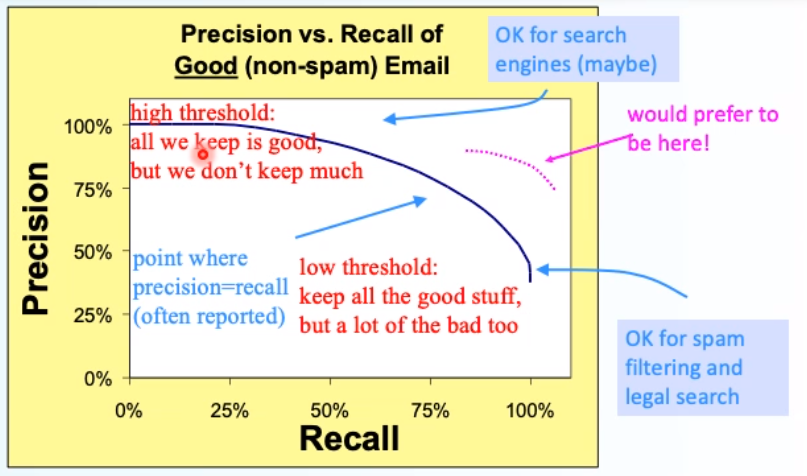
\includegraphics[scale=0.5]{10.png}
\end{center}
\begin{center}
	Contingency table\\
	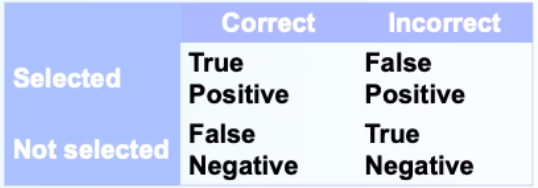
\includegraphics[scale=0.5]{11.png}
\end{center}
\paragraph{Micro vs Macro Averaging} Macro: performance for each class.\\
Micro: decision for all classes, compute contingecy table and evaluate
\paragraph{Multiclass Classification} More than 2 class, a binary classifier to dinstiguish belongin to a class and \textit{not belonging} to it.
\paragraph{Training Size} The more the better, usually.
\paragraph{Violation of Naive Bayes Assumptions} Conditional and positional independence.\\
Naive Bayss is not so naive. Among state of the art algorithms, being robust to irrelevant features (cancel each others). A good baseline for text classification, but not the best.\\
Optimal if the independence assumptions hold. Also is very fast, low storage requirements and \textbf{online learning algorithm} (incremental training, on new examples).
\paragraph{Example: SpamAssassin} Naive Bayes widely used in spam filtering.
\section{•}
\paragraph{Regular Expressions}
Formal language for specifying text strings. Letters inside square brackets, or specified ranges, like [] and [A-Z], or negations.
\paragraph{Tokenization} To do before analysis, for information retrieval and extraction, and spell-checking. Three tasks:\begin{enumerate}	
	\item Segmenting/tokenizing words in running text
	\item Normalizing word formats
	\item Segmenting sentences in running text
\end{enumerate}
\subparagraph{What's a Word?} Not easy. Babbling, in spoken language, or "are \textit{cat} and \textit{cats} the same word?".\\
Terminology:
\begin{list}{}{}
	\item \textbf{Lemma}: a set of lexical forms having the same stem, major part of speect, and rough word sense. What you would find in a dictionary.\\
	\textit{Cat} and \textit{cats} = same lemma
	\item \textbf{Wordform}: full inflected surface form.\\
	\textit{Cat} and \textit{cats} = different wordform
	\item \textbf{Type}/Form: element of the vocabulary
	\item \textbf{Token}: an instance of that type during text
\end{list}
How many words? $N$ tokens and $V$ vocabulary, set of types (of size $|V|$)\\$|V|>O(N^{\frac{1}{2}})$\\
Google N-grams has $N = 1$ trillion and $|V| = 13$ million.
\paragraph{Stanza Tokenizer} Toolkit, ternary classifier to distinguish between: normal character, end of token and end of sentence.
\paragraph{Clitics} Some languages have composite words: lascia-mi, lascia-me-lo\ldots Splitting clitics is important for parsing, since clitics incorporate relevant syntactic components (e.g. pronouns corresponding to an object of the verb).\\
Train 4-class tokenizer: normal character, end of token, end of sentence, start of clitic.
\section{Classification}
\begin{enumerate}
	\item Define classes/categories
	\item Label text
	\item Extract features
	\item Select classifier: Naive Bayes Classifiers, Decision Trees, SVMs, Neural Networks\ldots
	\item Train it
	\item Use it to classify new examples
\end{enumerate}
The data is easier to handle if it's linearly separable. Naive Bayes is slightly more general than DTs.
\paragraph{Naive Bayes} Simple model, can scale easily to millions of training examples, efficient and fast in training and classification.\\
A major limitation is the independence assumption, which has two consequences: the linear ordering of words is ignored (bag of words model) and the words are independent of each other given the class.\\
It's an inappropriate assumption if there are strong conditional dependencies between the variables. Classifiers may end up "double-counting" the effect of highly correlated features, pushing the classifier closer to a given labeled than is justified.
\paragraph{Decision Trees} Capable to generate understandable rules, and perform classification without requiring much computation. Can handle continuous and categorical variables and provide clear indication of the important features.\\
But it's prone to errors in classification problems with many classes and small numbers of training examples. Also can be computationally expensive to train: need to compare all possible splits, and pruning can be expensive.
\paragraph{Linear vs non-linear algorithms} We find out if data is linearly or non linearly separable only empirically.\\
Linear algorithms, when data is linearly separable, are simpler and uses less parameters, but high dimensional data (like for NLP) usually isn't linearly separable. For non linearly separable data, non linear algorithms are more accurate, although more complicated and with more parameters, like kernel methods.
\subsection{Linear Binary Classification}
Data: $\{(x_i,y_i)\}$ for $i=1,\ldots,n$\begin{list}{}{}
	\item $x \in R^d$
	\item $y \in \{-1,+1\}$
\end{list}
Question: find a linear decision boundary $$wx + b$$ an hyperplane such that the classification rule associated with it has minimal probability of error.\\
Classification rule: $$y = sign(wx+b)$$
\paragraph{Perceptron} Solves if linearly separable. Basic idea: go through all existing data patterns whose label is known, if correct continue. If not, add to the weights a quantity proportional to the product of the input pattern with $y$ ($-1$ or $+1$)
\subsection{Hidden Markov Models}
\paragraph{Markov Chain} Stochastic model describing a sequence of possible events in which the probability of each event depends only on the state attained in the previous event.
\begin{center}
	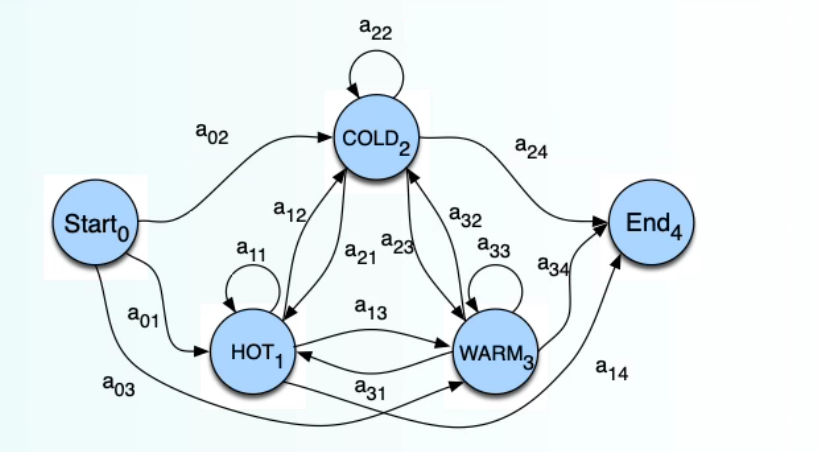
\includegraphics[scale=0.5]{12.png}
\end{center}
%salta il resto
\paragraph{Hidden Markov Model} For the chains, the output symbols are the same as the states. In named-entity or part-of-speech tagging (and speech recognition) the output symbols are \textbf{words} and the hidden states are \textbf{something else}: POS tags, named-entity tags.\\
So we need an extension: a \textbf{hidden Markov model} is an extension of a Markov chain in which the input symbols are not the same as the states. This means \textbf{we don't know which state we're in}.
\subparagraph{Example: speech} Observed outputs are phones (speech sounds) and hidden states are phonemes (units of sound).\\
Loopbacks because a phone is circa 100ms but phones are captured every 10ms, so each phone repeats 10 times (simplifying greatly).
\begin{center}
	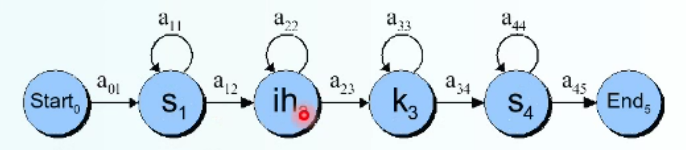
\includegraphics[scale=0.5]{14.png}
\end{center}
\begin{center}
	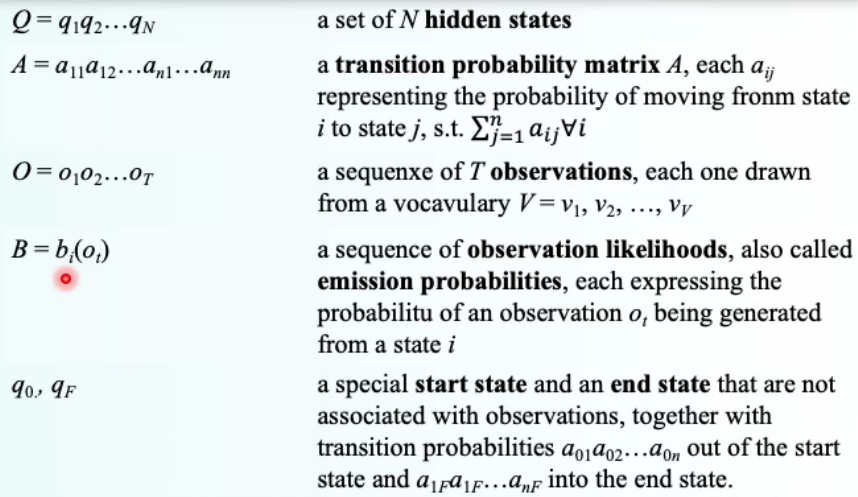
\includegraphics[scale=0.5]{13.png} %TODO riscrivere
\end{center}
\paragraph{Markov Assumption} $$P(q_i\:|\:q_1,\ldots,q_{i-1} = P(q_i\:|\:q_{i-1})$$
\paragraph{Output-independence assumption} $$P(o_t\:|\:O_1^{t-1},q_1^t)P(o_t\:|\:q_t)$$
\paragraph{Three basic problems}
\begin{list}{}{}
	\item \textbf{Evaluation}: given the observation sequence $O = (o_1,\ldots,o_T)$ and a HMM model $\Phi = (A, B)$, how to efficiently compute $P(O\:|\:\Phi)$ the probability of the observation sequence given the model?
	\item \textbf{Decoding}: given the observation sequence $O = (o_1,\ldots,o_T)$ and an HMM model $\Phi = (A, B)$, how do we choose a corresponding state sequence $Q = (q_1,\ldots,q_T)$ that is optimal in some sense (i.e. best explains the observations)?
	\item \textbf{Learning}: how do we adjust the model parameters $\Phi = (A,B)$ (transition and emission probabilities) to maximise $P(O\:|\:\Phi)$?
\end{list}
\paragraph{Computing the likelihood} Given an HMM $\lambda = (A, B)$ and an observation sequence $O$, determine the likelihood $P(O, \lambda)$.
$$P(O\:|\:Q)=\prod_{i=1}^T P(o_i\:|\:q_i)$$
$$P(O,Q) = P(O\:|\:Q)\cdot P(Q) = \prod_{i=1}^T P(o_i\:|\:q_i)\cdot\prod_{i=1}^n P(q_i\:|\:q_{i-1})$$
\subparagraph{Forward Algorithm} Dynamic programming algorithm: compute the likelihood of the observable sequence by summing over all possible hidden state sequences, but to do this efficiently we fold all the sequences into a single trellis. We compute $P(o_1,\ldots,o_T,q_T = q_F\:|\:\lambda)$ by recursion.\begin{list}{}{}
	\item $\alpha_t(j)$: cell of the forward algorithm trellis that represents the probability of being in state $j$ after seeing the first $t$ observations given the automaton.\\
	Thus the cell expresses the probability $$\alpha_t(j) = P(o_1,\ldots,o_T,q_T=j\:|\:\lambda)$$
	\item The recursion is as follows:
	\begin{enumerate}
		\item \textbf{Initialization} $$\alpha_1(j) = a_{0j}b_j(o_1)\:\:\:\:\:1\leq j\leq N$$
		\item \textbf{Recursion} (since states 0 and $F$ are non-emitting) $$\alpha_t(j) = \sum_{i=1}^N\alpha_{t-1}(i)a_{ij}b_j(o_t)\:\:\:\:\:1\leq j\leq N, 1<t\leq T$$
		\item \textbf{Termination} $$P(O\:|\:\lambda) =\alpha_T(q_F)=\sum_{i=1}^N\alpha_T(i)a_{iF}$$
	\end{enumerate}
\end{list}
\begin{center}
	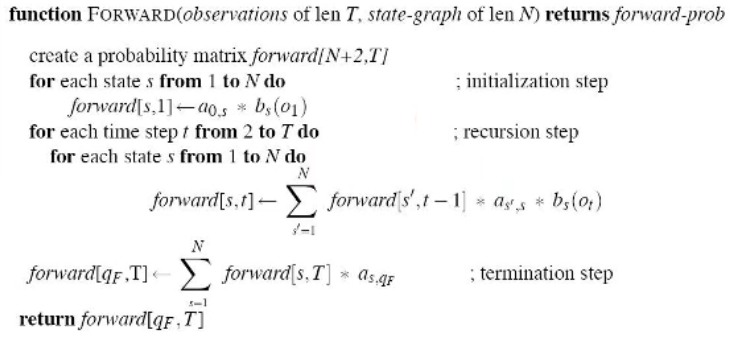
\includegraphics[scale=0.5]{15.png}
\end{center}
\paragraph{Decoding} Given an observation and a HMM, the task of the decoder is to find the best hidden state sequence.\\
Given the observation sequence $O = (o_1,\ldots,o_T)$, and a HMM $\Phi = (A, B)$, how to choose a corresponding state sequence $Q = (q_1,\ldots,q_T)$ that is optimal in some sense (i.e. best explains the observations)?\\
One possibility: for each hidden state sequence $Q$, compute $P(O\:|\:Q)$ and pick the highest, but we have $N^T$ possibilities.\\
Instead: \textbf{Viterbi algorithm}, dynamic programming algorithm that uses similar trellis as the Forward algorithm.
\paragraph{Viterbi Algorithm} We want to compute the joint probability of the observation sequence together with the best state sequence.
$$\max_{q_0,\ldots,q_T} P(q_0,\ldots,q_T,o_1,\ldots,o_T, q_T=q_F\:|\:\lambda)$$
$$v_t(j) = \max_{q_0,\ldots,q_T} P(q_0,\ldots,q_{t-1},o_1,\ldots,o_t, q_t=j\:|\:\lambda)$$
$$v_t(j) = \max_{i=1}^N v_{t-1}(i)a_{ij}b_j(o_t)$$
The recursion is as follows:
\begin{enumerate}
	\item \textbf{Initialization}
	$$v_1(j) = a_{0j}b_j(o_1)\:\:\:\:\:1\leq j\leq N$$
	$$bt_1(j) = 0$$
	\item \textbf{Recursion} (recall that states 0 and $q_F$ are non-emitting)
	$$v_t(j) = \max_{i=1}^N v_{t-1}(i)a_{ij}b_j(o_t)\:\:\:\:\:1\leq j\leq N, 1<t\leq T$$
	$$bt_t(j) = \arg\max_{i=1}^Nv_{t-1}(i)a_{ij}b_j(o_t)\:\:\:\:\:1\leq j\leq N, 1<t\leq T$$
	\item \textbf{Termination}\\
	Best score: $$P^* = v_t(q_F) = \max_{i=1}^N v_T(i)\cdot a_{iF}$$
	Start of backtrace: $$q_T^* = bt_T(q_F) = \arg\max_{i=1}^N v_T(i)\cdot a_{iF}$$
\end{enumerate}
Processes observations from left to right, filling out the trellis. Each cell $v_t(j) = \max_{i=1}^N v_{t-1}(i)a_{ij}b_j(o_t)$ is composed of:
\begin{list}{}{}
	\item $v_{t-1}(j)$ the \textbf{previous Viterbi path probability} from the previous time step
	\item $a_{ij}$ the \textbf{transition probability} from previous state $q_i$ to current state $q_j$
	\item $b_j(o_t)$ the \textbf{state observation likelihood} of the observation symbol $o_t$ given the current state $j$
\end{list}
\paragraph{Training a HMM} Baum-Welch algorithm (Expectation Maximization), no details.
\subsubsection{Part of Speech Tagging} The parts-of-speech, or lexical categories/word classes/lexical tags/POS, are nouns, verbs, adjectives, prepositions\ldots we'll use the term POS the most. Examples:
\begin{list}{}{}
	\item N, noun
	\item V, verb
	\item ADJ, adjectives
	\item ADV, adverbs
	\item \ldots
\end{list}
For example, "the koala put the keys on the table" $\rightarrow$ "DET N V\ldots"\\
But words often have more than one POS: "back" can be ADJ, ADV, N, V. POS tagging problem is determining the POS tag for a particular instance of a word.\\
We want, out of all sequences of $n$ tags $t_1,\ldots,t_n$, the single tag sequence such that $P(t_1,\ldots,t_n\:|\:w_1,\ldots,w_n)$ is the highest $$\hat{t}_1^n=\arg\max_{t_1^n} P(t_1^n\:|\: w_1^n)$$
We can compute it using the Bayes rule to transform it into a set of other probabilities that are easier to compute.
$$\hat{t}_1^n=\arg\max_{t_1^n} P(w_1^n \:|\: t_1^n)P(t_1^n)$$
Excluding the denominator because we're taking the maximum. It's composed by likelihood and prior\begin{list}{}{}
	\item Likelihood $P(w_1^n \:|\: t_1^n) \simeq \prod_{i=1}^n P(w_i\:|\:t_i)$ with the naive Bayes assumption
	\item Prior $P(t_1^n)\simeq \prod_{i=1}^n p(t_i\:|\:t_{i-1})$ with the Markov assumption 
\end{list}
\paragraph{Two kinds of probabilities}
\begin{list}{}{}
	\item Tag transition probabilities $P(t_i\:|\:t_{i-1})$\\
	The probabilities that a given tag $t_i$ is preceded by another given tag $t_{i-1}$.
	\item Word likelihood probabilities $P(w_i\:|\:t_i)$\\
	The probability that given a tag $t_i$, it corresponds to the word $w_i$
\end{list}
\subsubsection{Sequence Tagging} For example classifying each token independently using information about the surrounding tokens (sliding window) as input features.\\
For sequence tagging, sequence models work better: HMMs, MEMMs, conditional random fields, convolutional neural networks\ldots
\paragraph{Discriminative Model} Estimate $P(y\:|\:x)$ in order to predict $y$ directly from $x$
$$\hat{y}=\arg\max_y P(y\:|\:x)$$
For example: max entropy, logistic regression, Conditional Random Fields, Support Vector Machines, CNNs\ldots
\paragraph{Generative Model} Use the Bayes rule to obtain $P(y\:|\:x)$ and use argmax for classification
$$\hat{y} = \arg\max_y P(y)P(x\:|\:y)$$
For example: naive Bayes, HMMs\ldots
\begin{multicols}{2}
\paragraph{Naive Bayes} Compute $$\hat{c}_j=\arg\max_j P(c_j\:|\:x)$$ using the Bayes rule $$\hat{c}_j = \arg\max_j P(c_j)P(x\:|\:c_j)$$
\columnbreak
\paragraph{Logistic Regression} Compute the posterior probability directly
$$P(c_j\:|\:x) = \frac{e^{w_jx}}{\sum_ie^{w_ix}}=\hbox{Sofmax}_j(w_jx)$$
$$\hat{c}_j = \arg\max_j P(c_j\:|\:x)$$
\end{multicols}
In the logistic regression we represent the input $x$ as a vector of features $f_i$
$$P(c_j\:|\:x) = \frac{e^{w_jf}}{\sum_ie^{w_if}}=\hbox{Sofmax}_j(w_jf)$$
For example:\begin{list}{}{}
	\item $f_1(c,x)=\left\{\begin{array}{l l}
	1&\hbox{if }word_i=\hbox{"race"}\wedge c=\hbox{NN}\\
	0&\hbox{else}
	\end{array}\right.$
	\item $f_4(c,x)=\left\{\begin{array}{l l}
	1&\hbox{if is\_lower\_case(}word_i\hbox{)}\wedge c= \hbox{VB}\\
	0&\hbox{else}
	\end{array}\right.$
	\item \ldots
\end{list}
\paragraph{Problems} Using Classifiers for Sequence Labeling presents some problems. It's not easy to integrate information from hidden labels on both sides. We make an hard decision on each token, when we should rather choose a global optimum: the best labeling for the whole sequence, and keeping each local decision as just a probability, not a hard decision.\\
Probabilistic sequence models allow integrating uncertainty over multiple, interdependent classifications and collectively determine the most likely global assignment. Some common approaches are: HMMs (Hidden Markov Models), CRFs (Conditional Random Fields), MEMMs as simplified versions of CRFs, RNNs\ldots
\paragraph{MEMM} HMM works backwards from the tags to the outputs, while a Maximum Entropy Markov Model works backwards: from the words to the probabilities of the tags. An MEMM is a discriminative model that extends a standard maximum entropy classifier by assuming that the unknown values to be learned are connected in a Markov chain.
$$P(q_1,\ldots,q_N\:|\:o_1,\ldots,o_N)=\prod_t^N P(q_t\:|\:q_{t-1},o_t)$$
The probability of a certain label $s$ is modeled in the same way as a maximum entropy classifier $$P(q\:|\:q',o)=\frac{e^{w\cdot f(o,q)}}{\sum_{o,q'}e^{w\cdot f(o,q')}}=\hbox{Softmax}_{o,q}(w\cdot f(o,q))$$
where $f(o,q)$ is a vector of joint $(o,q)$ features and $w$ are the corresponding weights.
\begin{center}
	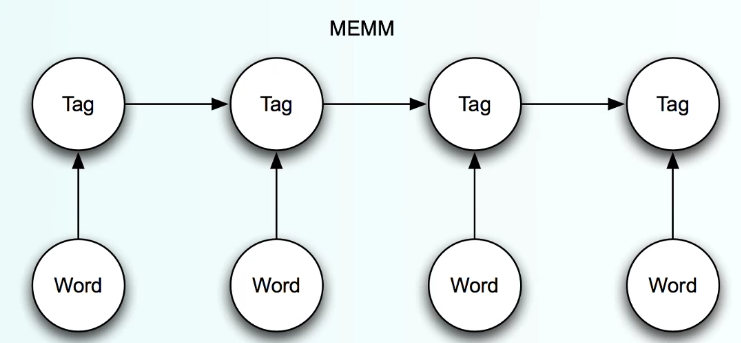
\includegraphics[scale=0.5]{16.png}
\end{center}
$$P(T\:|\:W) = \prod P(t_i\:|\:t_{i-1}, w_i)$$
We can also add \textbf{features} and use them in computing the probabilities.
\begin{center}
	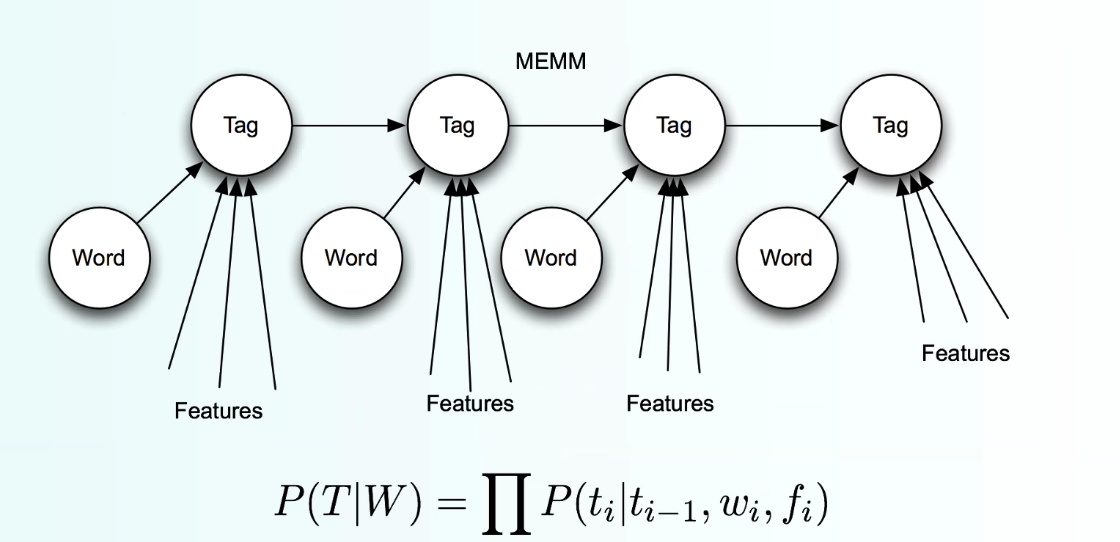
\includegraphics[scale=0.33]{17.png}
\end{center}
\begin{center}
	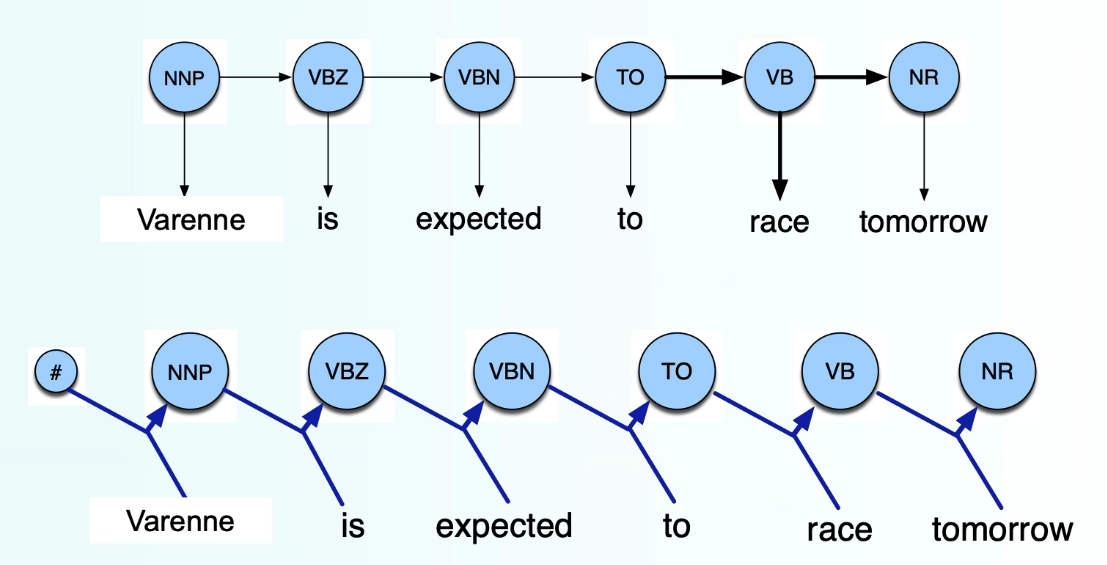
\includegraphics[scale=0.33]{18.png}\\
	An example of HMM vs MEMM
\end{center}
Viterbi algorithm can be used to select sequence of tags optimal given the whole sentence. In MEMM, decoding via Viterbi is
$$v_t(j) = \max_{i=1} v_{t-1}(i)P(q_j\:|\:q_i, o_t)\:\:\:\:\hbox{ for } 1\leq j\leq N, 1< t\leq T$$
\begin{center}
	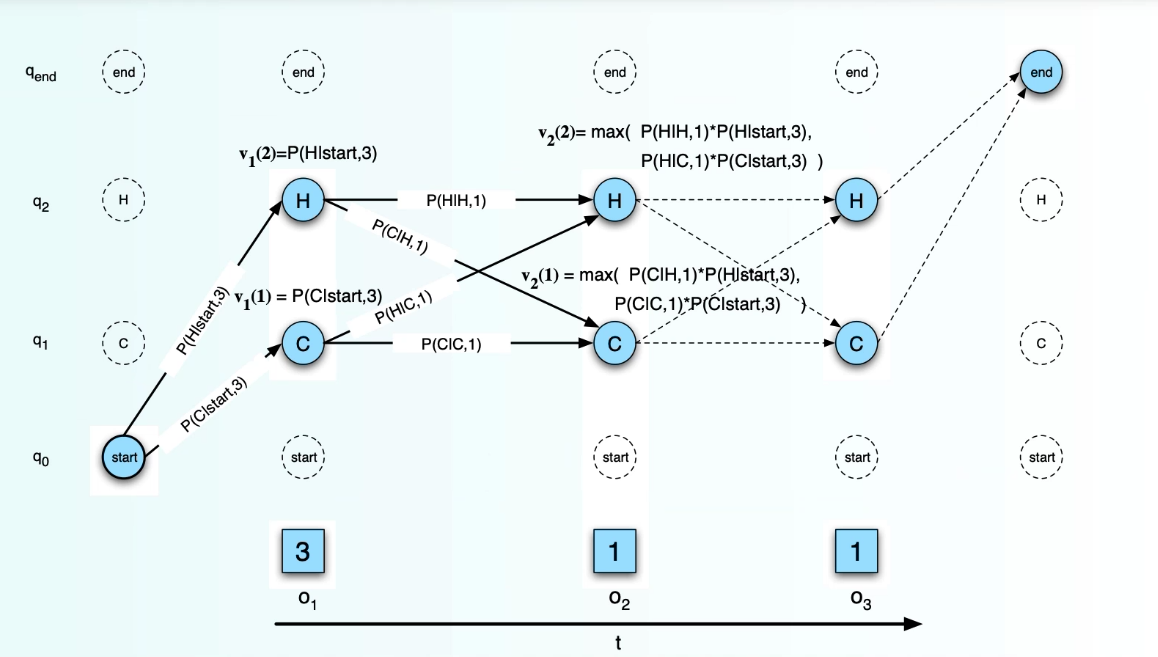
\includegraphics[scale=0.5]{19.png}
\end{center}
\subsubsection{Named Entity Tagging}
Given a text, find the entities with proper names: person names, city names\ldots the "capitalized things". Typical approach is based on rules, might not be accurate enough. An approach based on ML needs training data, labeling them and using a classifier. Labeling may be easy: annotate each word, but an entity may span more words (name and surname, for example) or be non-continguous, overlapping with other words and perhaps other named entities (examples in biomedical entities).\\
Typical, named entities systems handle very few categories:
\begin{center}
	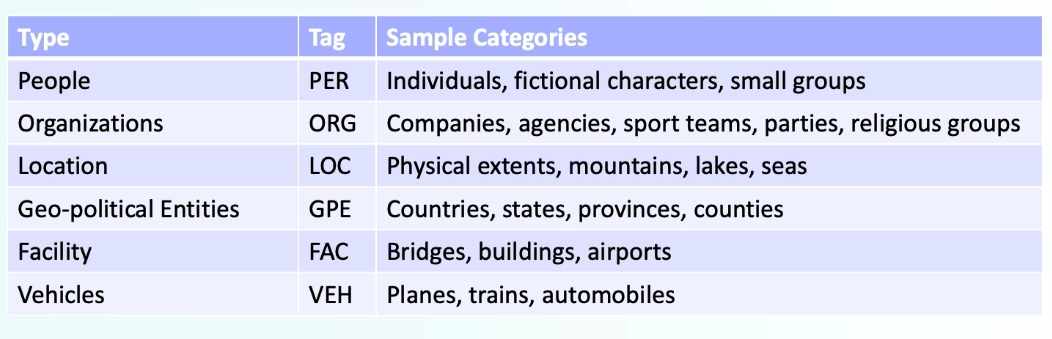
\includegraphics[scale=0.33]{20.png} %TODO rewrite
\end{center}
\paragraph{Approaches} As with partial parsing and chinking, there are two basic approaches (and hybrids):
\begin{list}{}{}
	\item \textbf{Rule-based}: patterns to mach things that look like names and environments that classes of names tend to occur in (regular expressions)
	\item \textbf{ML-based}: get annotated data, extract features and train systems to replicate the annotation. Typical approach today
\end{list}
\begin{center}
	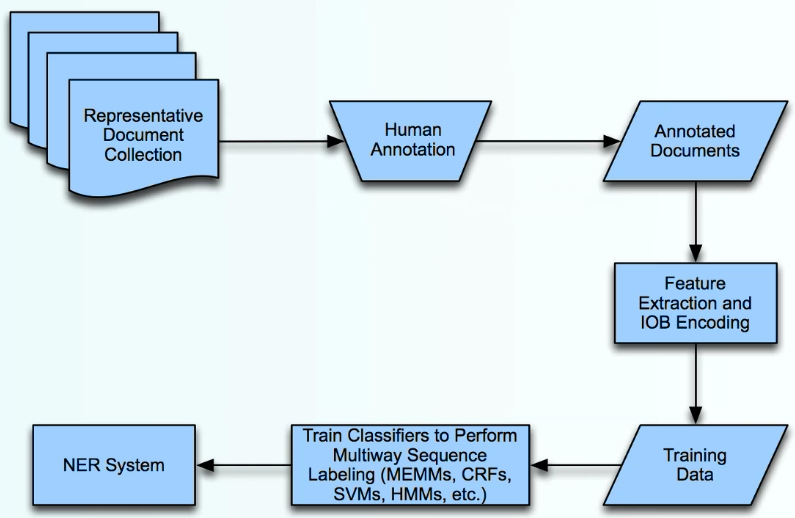
\includegraphics[scale=0.33]{21.png}
\end{center}
For $N$ classes we have $2N + 1$ tags, with IOB encoding: an I and a B for each tag.
\begin{center}
	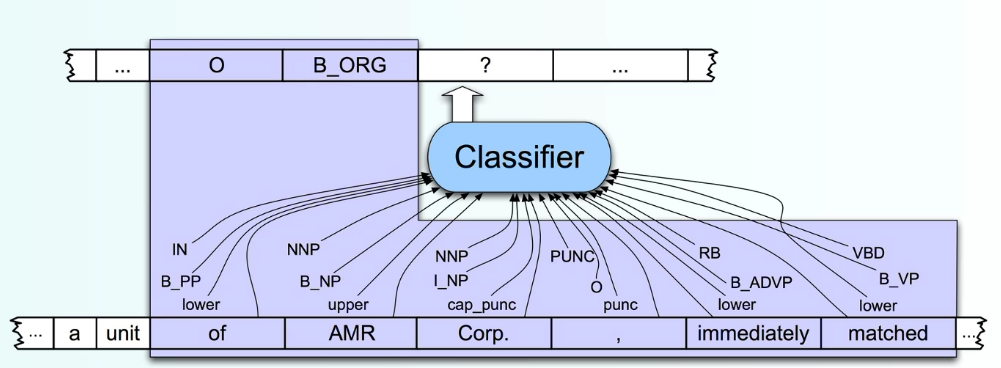
\includegraphics[scale=0.5]{22.png}
\end{center}
Summary of the approaches.
\section{Convolutional Neural Networks for NLP}
The main CNN idea is to compute vectors for every poissible word subsequence of a certain length, regardless of whether the phrase is grammatially correct, and group them afterwards. Not very linguistically nor cognitively plausible.\\
Convolution is classically used to extract features from images
$$(f * g)(n) = \sum_{m=-M}^M f(n-m)g(m)$$
Much like a "sliding window" across the data.
\begin{center}
	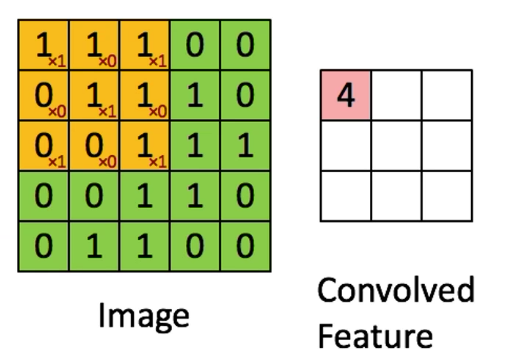
\includegraphics[scale=0.5]{23.png}
\end{center}
A convolutional layer in a NN is composed by a set of filters: combines a local selection of input values into an output value, sweeping across all input.\\
During training each filter specializes into recognizing some kind of relevant combination of features. CNNs work well on stationary features (independent from position). Filters have additional parameters that define:\begin{list}{}{}
	\item Behavior at the start/end of documents (\textbf{padding})
	\item Size of the sweep step (\textbf{stride})
	\item Possible presence of holes in the filter window (\textbf{dilation})
\end{list}
\paragraph{Distant Supervision} Use the convolutional neural network to further refine the embeddings: word embeddigns from plain text are completely clueless about their sentiment behavior. Collect 10M tweets containing positive emoticons, used as distantly supervised labels to train sentiment-aware embeddings.
\paragraph{Sentiment Specific Word Embeddings} The idea is to build sentiment specific word embeddings where we return also the polarity of the word: positive, neutral or negative.\\
Sentiment Specific Embeddings are learned:
\begin{list}{}{}
	\item The generic loss function is $L_{CW}(x, x^c) = \max(0, 1-f_\theta(x)_0 + f_\theta(x^c)_0)$
	\item The SS loss function is
	$$L_{SS}(x, x^c) = \max(0, 1 - d_s(x)f_\theta(x)_1 + d_s(x^c)f_\theta(x^c)_1)$$
	$$L(x,x^c) = \alpha L_{CW}(x,x^c)+(1-\alpha)L_{SS}(x,x^c)$$
	With gradients
	$$\left(\begin{array}{c}
	\frac{\partial L}{\partial f_\theta(x)}\\
	\frac{\partial L}{\partial f_\theta(x^c)}
	\end{array}\right)_0 = \left\{\begin{array}{cl}
	\left(\begin{array}{c}
	-1\\1
	\end{array}\right)&\hbox{if }L_{CW}(x, x^c) > 0\\
	\left(\begin{array}{c}
	0\\0
	\end{array}\right)&\hbox{else}\\
	\end{array}\right.$$
\end{list}
With $x$ sentence, $x^c$ corrupted sentence obtained by replacing the center word with a random word, $f(x)\in \{0,1\}^2$ is the function computed by the network and $d_s(x)\in\{1,-1\}$ represents the polarity of $x$.
\paragraph{Sentiment Classification from a Single Neuron} A char-level LSTM with 4096 units has been trained on 82M reviews from Amazon, only to predict the next character. After training, one of the units had a very high correlation with sentiment, resulting in \textbf{state-of-the-art accuracy when used as a classifier}. The model can also be used to generate text: by setting the value of the sentiment unit, one can control the sentiment of the resulting text.
\subsection{Regularization} 
We can use \textbf{dropout}: creating a masking vector $r$ of Bernoulli random variables with probability $p$ (hyperparameter) of being 1 and delete features during training $$h = W(r\otimes z) + b$$
Prevents overfitting. Not used at test time, scaling final vector by probability $p$. Usually yields an accuracy increase of 2-4\%.
\section{Recurrent Neural Networks}
Up until now, whether we grouped words or not each word/group would be handled independently from the others.
\paragraph{Recap} A language model assigns to each sentence $W$ a probability $P(W) = P(w_1,\ldots,w_n)$. Alternatively we want to compute $P(w_n\:|\:w_1,\ldots,w_{n-1})$.\\
The model that computes either probability is called \textbf{Language Model}, and language modeling is the task of estimating a language model.\\
The Markov assumption is that $w_n$ depends only on the preceding $n-1$ words. $n$-gram models have sparsity (out-of-vocabulary words and never-seen-prefixes) and storage problems (counts for every $n$-gram): bigger $n$ makes the sparsity problem words, typically $n<5$.\\
\textbf{Neural Language Models} improves over $n$-gram language models: no sparsity and no need to store all observed $n$-grams, but still problems: fixed window is too small, never large enough, and no symmetry in the input where each word is still treated independently and multiplied by completely different weights. We need a \textbf{neural architecture that can process any length input}.
\paragraph{Recurrent} Because they perform the same process for every element where \textbf{the output depends on the previous elements}. RNNs have a "memory" which captures information about what has been calculated so far. In theory, RNNs can make use of information in arbitrarily long sequences.
\begin{center}
	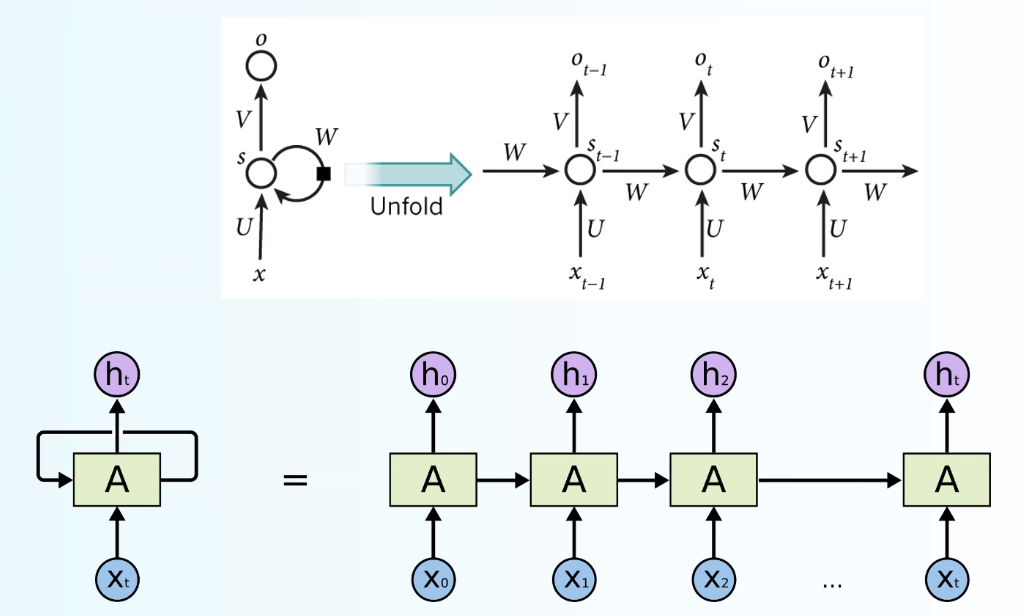
\includegraphics[scale=0.5]{24.png}
\end{center}
\paragraph{Hidden Units} The hidden state $s_t$ represents the memory of the network: it captures information about what happened in all the previous time steps.\\
The output $o_t$ is computes solely based on the memory at time $t$.\\
$s_t$ typically can't capture information from too many time steps ago. Unlike traditional deep networks, which uses different parameters at each layer, a RNN shares the same parameters across all steps ($U, V$ and $W$ above). This reflects the fact that we are performing the same task at each step, just with different inputs, greatly reducing the total number of parameters we need to learn.
\paragraph{Advantages} We can process input of any length and model size doesn't increase with longer input. The computation for step $t$ in theory can use information from many steps back.\\
Weights are shared across timesteps, so representations are shared too.
\paragraph{Disadvantages} Recurrent computation is really slow. In practice, is difficult to access information from many steps back.
\paragraph{Simple RNN Language Model}
\begin{center}
	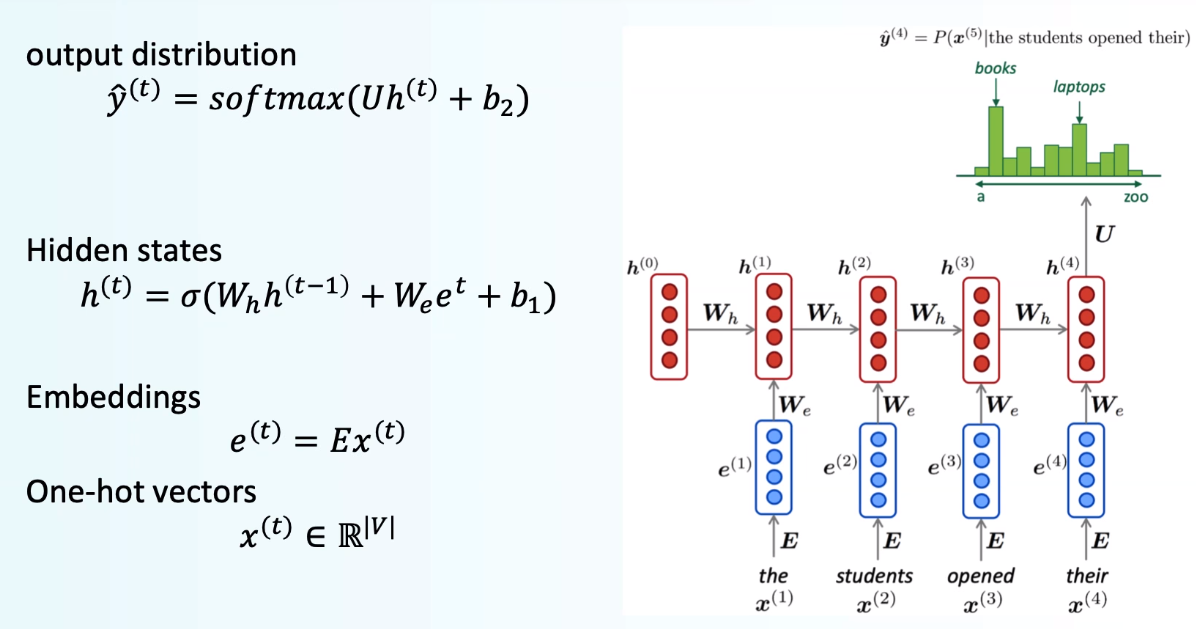
\includegraphics[scale=0.5]{25.png}
\end{center}
\paragraph{Vanilla RNN}
\begin{center}
	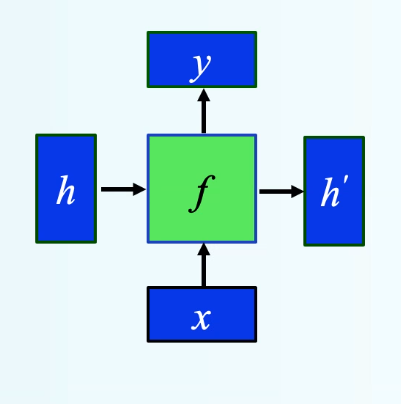
\includegraphics[scale=0.5]{26.png}
\end{center}
$$h_t = \sigma\left(Wh_{t-1} + Wx_t + b\right)$$
$$y_t = \sigma\left(Vh_t\right)$$
Notice that $y$ is computed from the current $h'$ only.
\paragraph{Training} Tasks:
\begin{list}{}{}
	\item for each timestep of the input sequence $x$ we predeict the output $y$ synchronously
	\item for the input sequence $x$ we predict the scalar value of $y$ (e.g. at the end of the sequence)
\end{list}
Main method: \textbf{backpropagation}, reliable and controlled convergence, supported by most ML frameworks. Other methods: evolutionary methods, expectation maximization, particle swarm\ldots\\
\paragraph{Backpropagation through time}
\begin{center}
	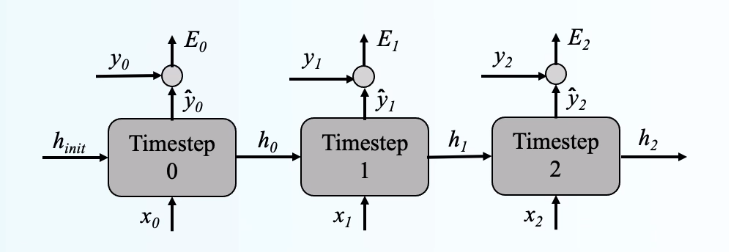
\includegraphics[scale=0.5]{27.png}
\end{center}
Applying the chain rule $$\frac{\partial h_2}{\partial h_0} = \frac{\partial h_2}{\partial h_1}\frac{\partial h_1}{\partial h_0}$$
For time 2:
$$\frac{\partial E_2}{\partial \Theta} = \sum_{k=0}^2\frac{\partial E_2}{\partial \hat{y}_2}\frac{\partial\hat{y}_2}{\partial h_2}\frac{\partial h_2}{\partial h_k}\frac{\partial h_k}{\partial\Theta}$$
\paragraph{Training RNN Language Model} Get a big corpus of text and feed into the RNN-LM, computing the output distribution for every step $t$.\\
Loss function on step $t$ is cross-exntropy between the predicted probability distribution $\hat{y}$ and the true next word $y^{(t)}$ (one-hot for $x^{(t+1)}$)
$$J^{(t)}(\Theta) = \hbox{CrossEntropy}(\hat{y}^{(t)}, y^{(t)}) = -\sum_{w\in V} y_w^{(t)}\log\hat{y}_w^{(t)} = -\log\hat{y}_{x_{t+1}}^{(t)}$$
Average this to get the overall loss for the entire training set
$$J(\Theta) = \frac{1}{T}\sum_{i=1}^T J^{(t)}(\Theta) = \frac{1}{T}\sum_{i=1}^T -\log\hat{y}_{x_{t+1}}^{(t)}$$
In practice: do this for each sentence and repeat through stochastic gradient descent.
\paragraph{Vanishing Gradients} Known problems: the gradients decay exponentially and networks stops learning without updating, making impossible to learn correlations between temporally distant events. A solution is to use ReLU instead of sigmoids.
\begin{center}
	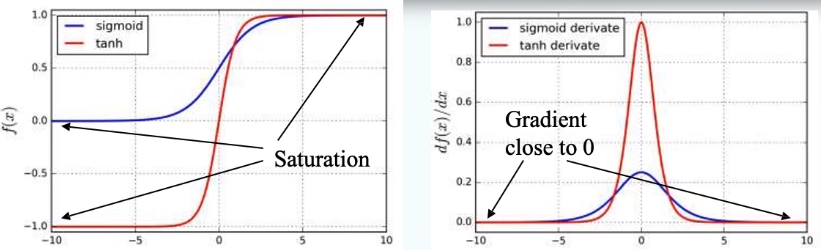
\includegraphics[scale=0.5]{28.png}
\end{center}
Smaller weights initialization leads to faster gradient vanishing, and very big initialization make the gradient diverge fast.
\paragraph{Exploding Gradients} The opposite: large increase in the norm, causing NaNs or large fluctuations in cost functions.
\begin{center}
	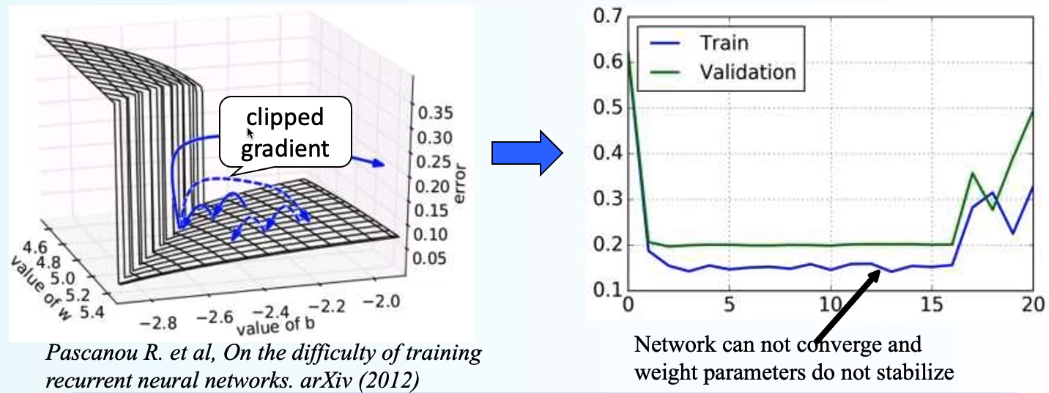
\includegraphics[scale=0.4]{29.png}
\end{center}
Solutions: gradient clipping, reducing learning rates or changing loss function by setting constraints on weights (L1 or L2 norms).
\subsection{Specializations}
\paragraph{Notation}\begin{center}
	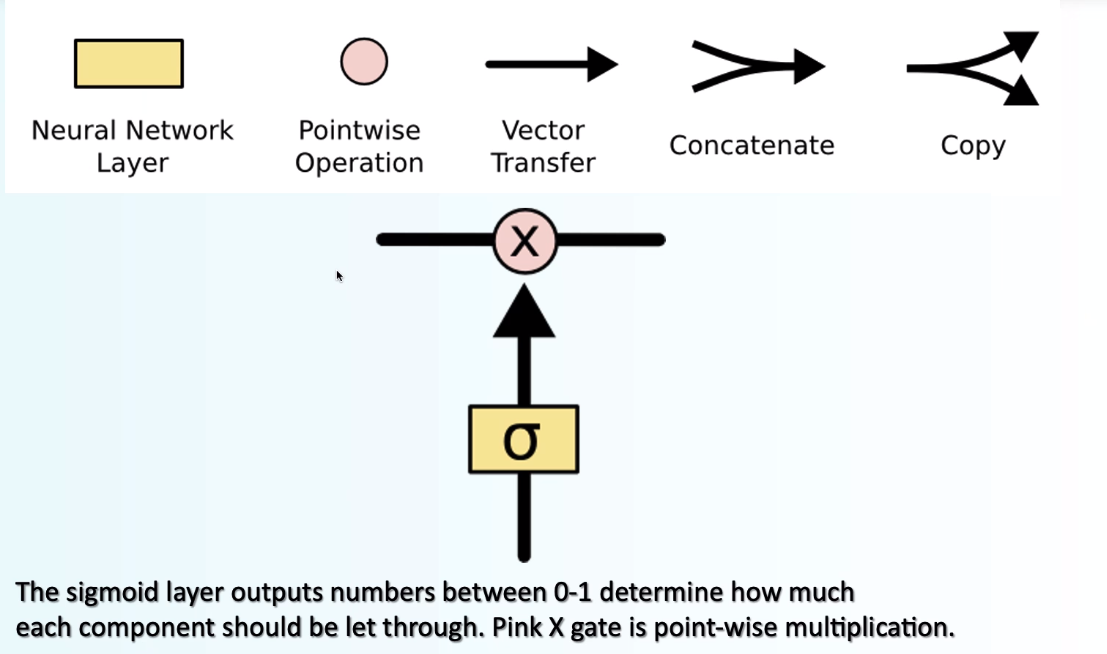
\includegraphics[scale=0.33]{30.png}
\end{center}
\subsubsection{LSTM}
\paragraph{Long Short-Term Memory}
\begin{center}
	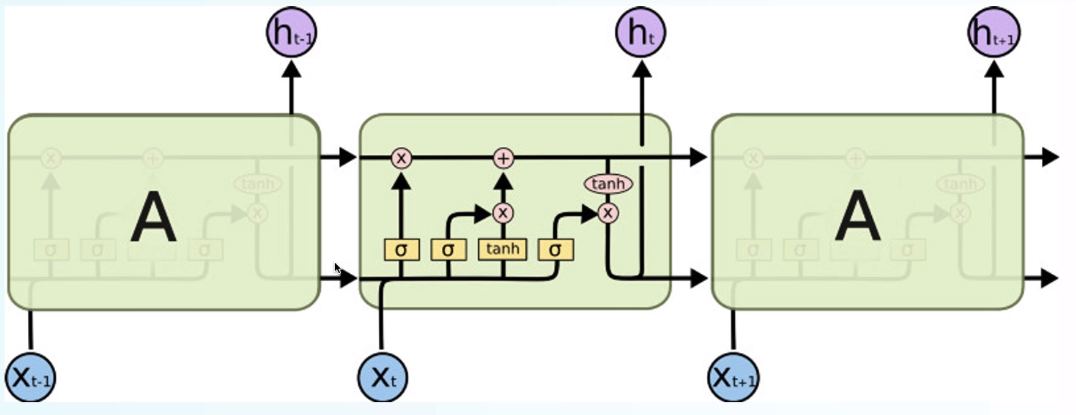
\includegraphics[scale=0.5]{31.png}
\end{center}
The core idea is this cells state $C_t$ is changed slowly with only minor interactions. Very easy for information to flow unchanged.
$$C_t = f_tC_{t-1}+i_t\hat{C}_t$$
The first sigmoid goes to the \textbf{forget gate}, determines how much information goes through.\\
the second sigmoid is the \textbf{input gate} and decides how much input is added in the cell state (so in the next pass).\\
The \textbf{output gate} of the third sigmoid controls what goes in the output.\\
Why sigmoid or tanh: sigmoid are used as 0/1 switches, and the vanishing gradients are already handled in the LSTMs.
\begin{center}
	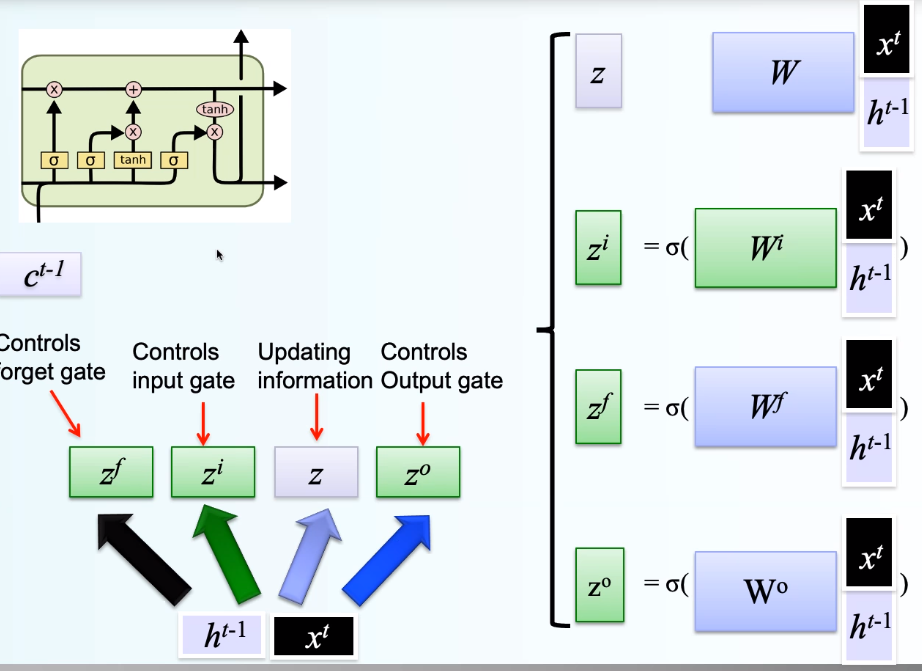
\includegraphics[scale=0.5]{32.png}
\end{center}
\begin{center}
	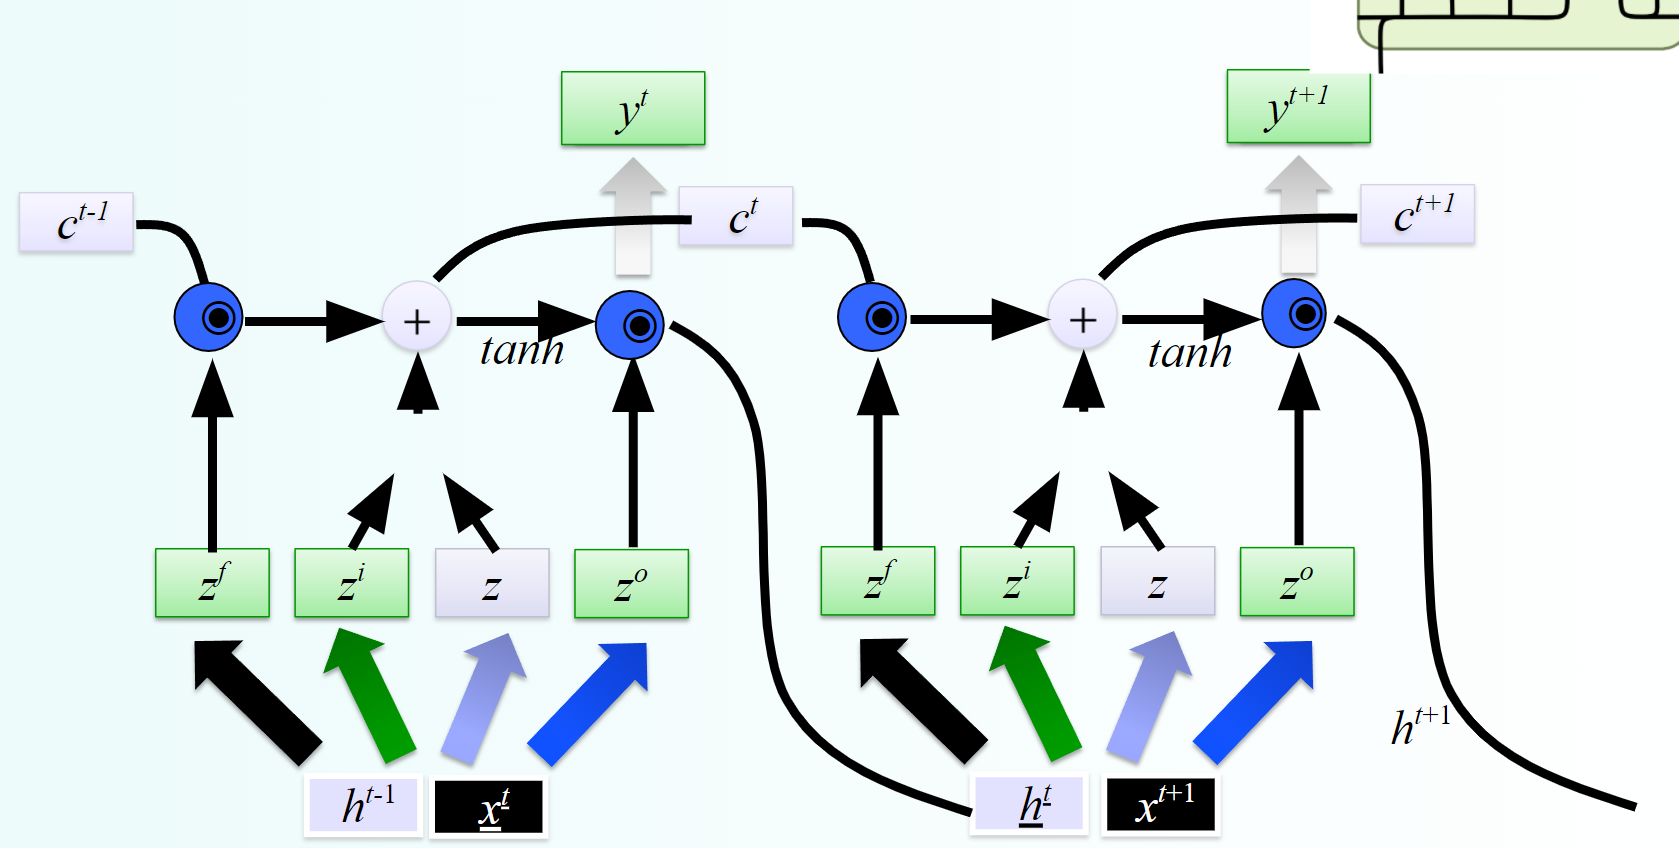
\includegraphics[scale=0.33]{35.png}
\end{center}
\subsubsection{GRU}
\paragraph{Gated Recurrent Units}
\begin{multicols}{2}
\begin{list}{}{}
	\item $z_t = \sigma(W_z\cdot[h_{t-1},x_t])$
	\item $r_t = \sigma(W_r\cdot[h_{t-1},x_t])$
	\item $\hat{h}_t = \tanh(W\cdot[r_t\cdot h_{t-1},x_t])$
	\item $h_t = (1-z_t)\cdot h_{t-1}+z_t\cdot\hat{h}_t$
\end{list}
\begin{center}
	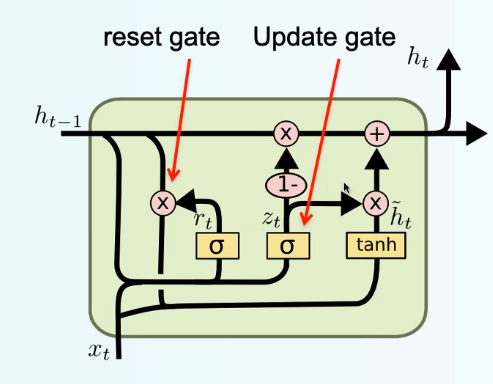
\includegraphics[scale=0.5]{33.png}
\end{center}
\end{multicols}
Combines forget and input gate into a single update gate, also merging cell state and hidden state. Simpler than LSTM.
\begin{center}
	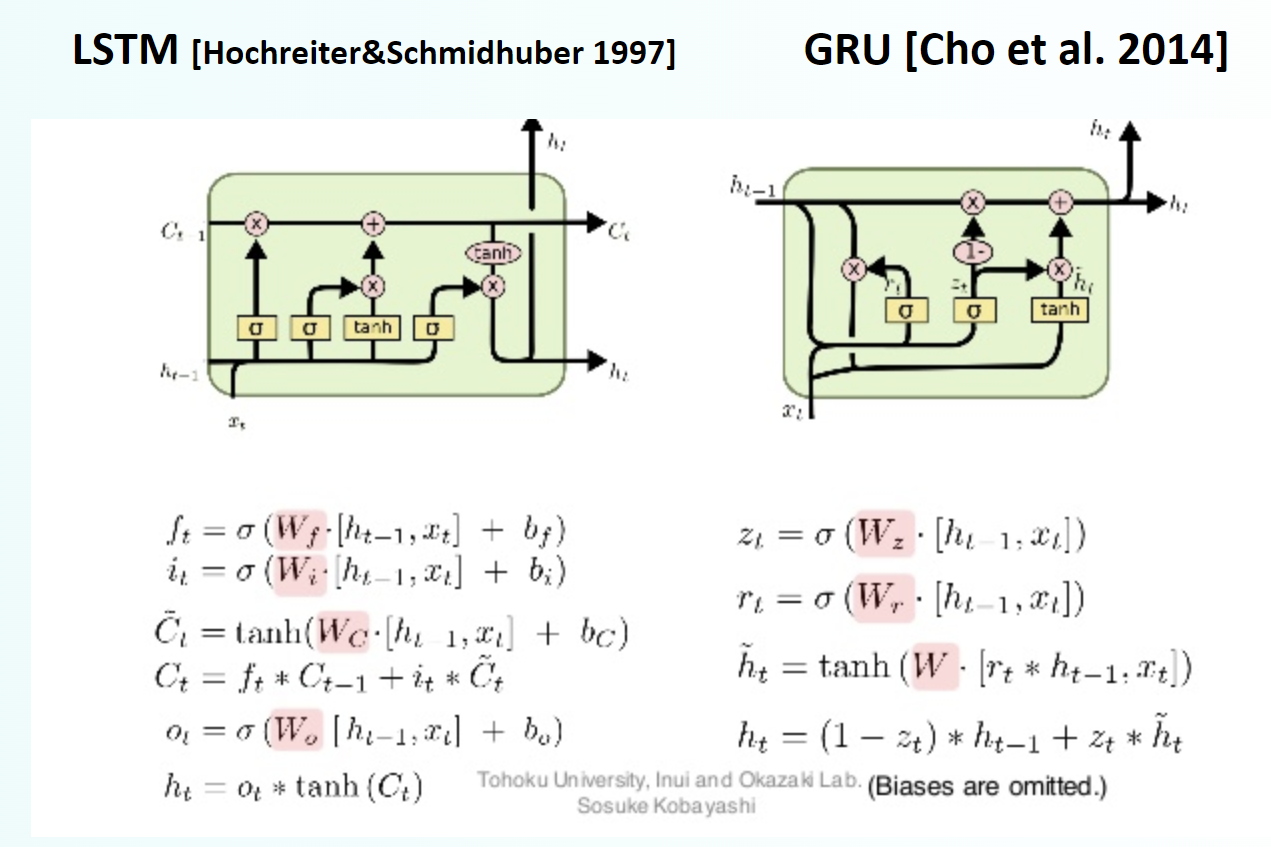
\includegraphics[scale=0.5]{34.png}
\end{center}
\section{Parsing}
\paragraph{Dealing with Text}
\begin{list}{}{}
	\item Bag Of Words representation: enough for classification and information retrieval
	\item N-Grams for language modeling, POS tagging\ldots
	\item Sequences for neural machine translations
\end{list}
But we have nothing that's applicable for information extraction or question answering.
\paragraph{Sentence Structure} Recovering the structure is needed to fully understand the language.\\
Syntax is the way words are arranged together into larger units, and grammar is a formalism used to describe the syntax of a language.\\
Structural ambiguity: prepositional attachment, coordination scope, verb phrase attachment.
\paragraph{Practical uses of parsing} \begin{list}{}{}
	\item \textbf{Relation Extraction}: knowledge graph enriched from relation extracted from dependency trees
	\item \textbf{Semantic Relation}
	\item \textbf{Translation}: helps disambiguating sentences
	\item \textbf{Sentiment Analysis}: improved by dependency parsing
	\item \textbf{Negation}: determining the scope of negations
	\item \textbf{Summarization}: detecting relevant parts
	\item \textbf{Question Answering}
\end{list}
In NLP we've seen information extraction and finding linguistic structure. Can be cast as \textbf{learning mapping}: strings to hidden state sequences (POS tagging), strings to strings (translation), strings to trees (\textbf{parsing}), strings to relational data structures (information extraction).
\subsection{Parsing Approaches}
\subsubsection{Constituency Grammar}
AKA phrase structure grammar or \textbf{context free grammar}.
\begin{center}
	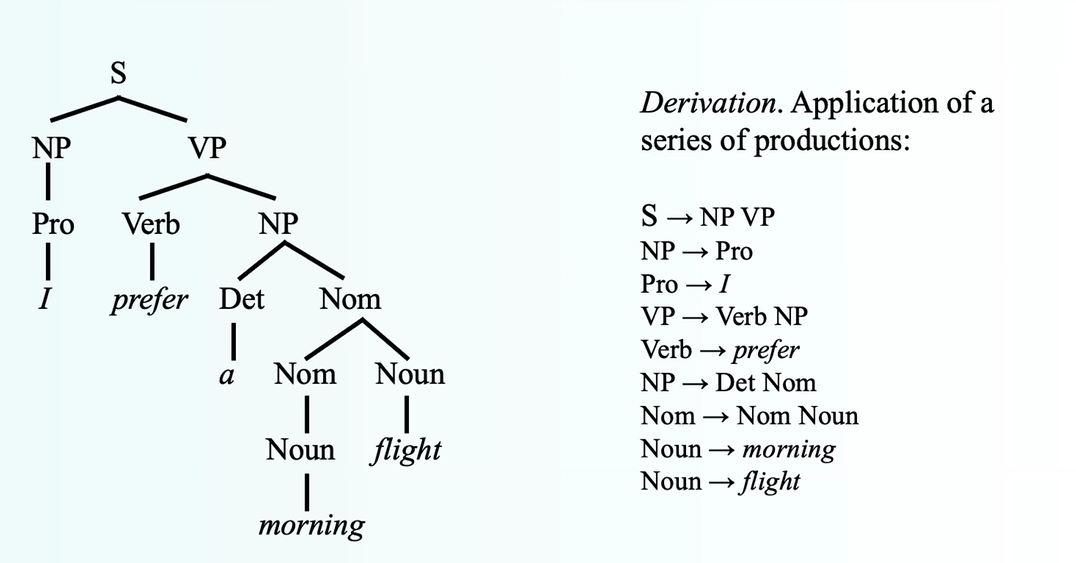
\includegraphics[scale=0.5]{36.png}
\end{center}
\paragraph{Context Free Grammars} $G = (N,\Sigma, R, S)$
\begin{list}{}{}
	\item Set of non-terminal symbols $N$
	\item Set of terminal symbols $\Sigma$ disjoint from $N$
	\item set of rules/productions $R$ in the form $A\rightarrow\beta$ with $A$ non-terminal, $\beta$ string of symbols from the infinte set of strings $(\Sigma\cup N)^*$
	\item A designated start symbol $S \in N$
\end{list}
$$L(G) = \{w\in \Sigma^*, S\rightarrow w\}$$
\paragraph{Constituency Parsing} Requires phase structure grammar and produces phrase structure parse tree.
\subparagraph{Statistical Parsing} Three components \begin{list}{}{}
	\item GEN is a function from a string to a set of candidate trees
	\item $\Phi$ maps a candidate to a feature vector
	\item $W$ is the parameter vector
\end{list}
Training by giving a set of sentences $X$ and the set of possible outputs (trees) $Y$ to learn a function $F_W:X\rightarrow Y$.\\
Parsing is choosing the highest scoring tree $$F_W(x)=\arg\max_{y\in GEN(x)}\Phi(y)\cdot W$$
% skip the details
\subsubsection{Dependency Grammar}
\paragraph{Dependency Structure} Shows which words depend on (modify or are arguments of) which other words. The syntactic structure of a sentence is described only in terms of the words in a sentence and a set if directed binary grammatical relations among the words.
\paragraph{Difference Between Constituency Tree and Dependency Trees}
\begin{center}
	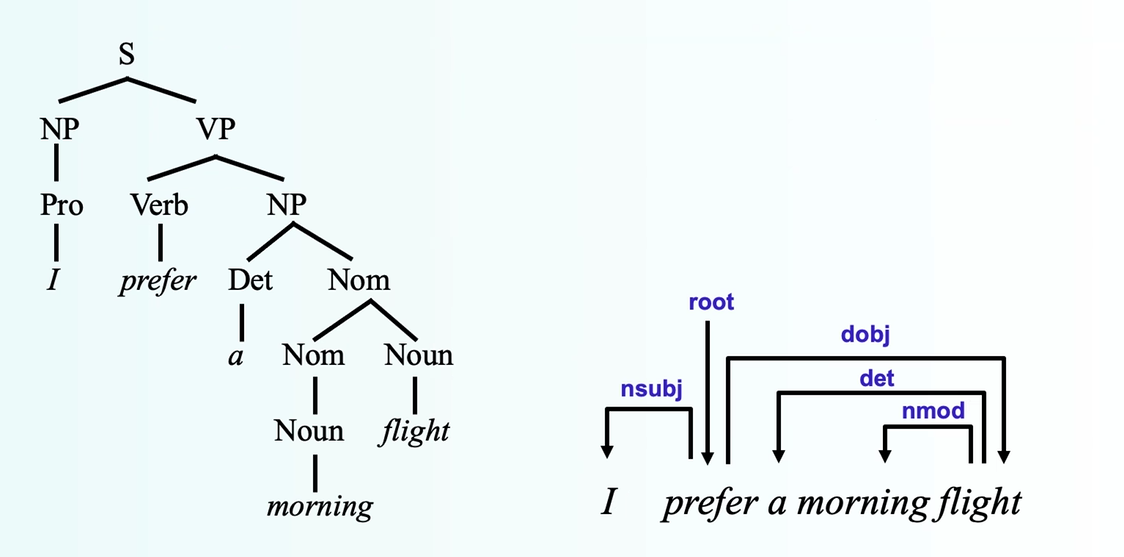
\includegraphics[scale=0.5]{37.png}
\end{center}
Criteria for a syntactic relation between a head $H$ and a dependent $D$ in a construction $C$
\begin{list}{}{}
	\item $H$ determines the syntactic category of $C$ ($H$ can replace $C$)
	\item $H$ determines the semantic category of $C$ ($D$ specifies $H$)
	\item $H$ is obligatory and $D$ may be optional
	\item $H$ selects $D$ and determines whether $D$ is obligatory
	\item The form of $D$ depends on $H$
	\item The linear position of $D$ is specified with reference to $H$
\end{list}
\paragraph{Annotation Constraints} A dependency graph $D = (W, A)$ is a directed rooted tree
\begin{list}{}{}
	\item $D$ is weakly connected: $i,j\in V\Rightarrow i\leftrightarrow^* j$
	\item $D$ is acyclic: $i\rightarrow j \Rightarrow \neg(j\rightarrow^* i)$
	\item $D$ obeys the \textbf{single-head constraint}: $i\rightarrow j \Rightarrow \neg(i'\rightarrow j)\:\:\forall\:i'\neq i$
\end{list}
The single-head constraints causes problems in handling certain linguistic phenomena.
\paragraph{Data-Driven Dependency Parsing}
\begin{list}{}{}
	\item \textbf{Graph Based}: consider the possible dependency graphs and define a score selecting the best scoring one.
	\item \textbf{Transition Based}: define a transition system that leads to a parse tree while analyzing a sentence one word at a time.
	\item \textbf{Constraint Satisfaction}: edges are deleted that don't satisfy hard constraints.
\end{list}
\subparagraph{Transition-Based Shift-Reduce Parsing}
Traditional statistical parsers are trained directly on the task of tagging a sentence. Instead, a shift-reduce parser \textbf{learns the sequence of parse actions required to build the parse tree}. An inductive parser \textbf{doesn't require grammar}, while a traditional parser requires a grammar for generating candidate trees.
\paragraph{Parsing as Classification} Inductive dependency parsing, based on Shift/Reduce actions: Learn from annotated corpus which action to perform at each step.
\paragraph{Dependency Graph} Let $R = \{r_1,\ldots,r_m\}$ the set of dependency types (the tags we'll put on the links).\\
A dependency graph for a sequence of words $W = w_1,\ldots,w_n$ is a labeled directed graph $D = (W,A)$ where\begin{list}{}{}
	\item $W$ is the set of nodes, i.e. the word tokens in the input sequence
	\item $A$ is a set of labeled arcs $(w_i, w_j, r)$ with $w_i,w_j\in W$ and $r \in R$
	\item $\forall\:w_j\in W$ there is at most one arc $(w_i, w_j, r)\in A$
\end{list}
The parser build such a graph. Its state at each time is a triple $(S, B, A)$ where
\begin{list}{}{}
	\item $S$ is a stack of partially processed tokens
	\item $B$ is a buffer of remaining input tokens
	\item $A$ is the arc relation for the dependency graph
\end{list}
$(h,d,r)\in A$ represent an arc $h-r\rightarrow d$ tagged with relation $r$.
\paragraph{Arc Standard Transitions}
$$\hbox{Shift}\:\:\:\:\:\frac{\langle S, n|B, A\rangle}{\langle S|n, B, A\rangle}$$
$$\hbox{Left-Arc}_r\:\:\:\:\:\frac{\langle S|s, n|B, A\rangle}{\langle S, n|B, A\cup\{(n, s, r\}\rangle}$$
$$\hbox{Right-Arc}_r\:\:\:\:\:\frac{\langle S|s, n|B, A\rangle}{\langle S, s|B, A\cup\{(s,n,r)\}\rangle}$$
\paragraph{Parser Algorithm} Is fully deterministic, using a trained model to predict the next action, given a representation of the context current state.
\begin{lstlisting}
Input Sentence: (w1, w2, ... , wn)
  S = <>
  B = <w1, w2, ... , wn>
  A = {}
  while B != <> do
	 x = getContext(S, B, A)
	 y = selectAction(model, x)
	 performAction(y, S, B, A)
\end{lstlisting}
\paragraph{Oracle} The gold tree of each sentence can be used to suggest which actions to perform in order to rebuild such gold tree. There can be more than one possible sequence to produce the same parse tree.\\
An Oracle is an algorithm that given the gold tree for a sentence, produces a proper sequence of actions that a parser may use to obtain that gold tree from the input sentence.\\
Simplest Oracle: arc standard Oracle, emulates the parser knowing what the outcome should be, returning the correct action at each step. Works but cannot handle certain situation: e.g. non-projectivity situations.
\paragraph{Projectivity} An arc $w_i\rightarrow w_k$ is projective $\Leftrightarrow\forall j,i<j<k$ or $i>j>k$ we have $w_i\rightarrow^* w_j$, so no arc crosses that arc. A dependency tree is projective if and only if every arc is projective.\\
Intuitively: arcs can be drawn without intersections.
\paragraph{Arc-Standard Algorithm}\begin{list}{}{}
	\item Doesn't deal with non-projectivity
	\item Every transition sequence produces a projective dependency tree (soundness)
	\item Every projective tree is produces by some transition sequence (completeness)
	\item Fast deterministic linear algorithm: parsing $n$ words requires $2n$ transition.
\end{list}
\paragraph{Arc Eager Transitions}
$$\hbox{Shift}\:\:\:\:\:\frac{\langle S, n|B, A\rangle}{\langle S|n, B, A\rangle}$$
$$\hbox{Left-Arc}_r\:\:\:\:\:\frac{\langle S|s, n|B, A\rangle}{\langle S, n|B, A\cup\{(n, s, r\}\rangle}$$
$$\hbox{Right-Arc}_r\:\:\:\:\:\frac{\langle S|s, n|B, A\rangle}{\langle S|s, s|B, A\cup\{(s,n,r)\}\rangle}$$
(Connects without removing, to delay decision and keep words on the stack that might need further connections to children)
$$\hbox{Reduce}\:\:\:\:\:\frac{\langle S|s, B, A\rangle}{\langle S, B, A\rangle}$$
\paragraph{Non-Projective Transitions} \begin{list}{}{}
	\item 
\end{list}
\paragraph{Learning Procedure}
\begin{list}{}{}
	\item Go through each sentence in the treebank and extract the sequence of actions suggested by the oracle.
	\item Emulate the parser and at each parser state extract a context representation of the state, in terms of features.
	\item Provide the features as input and the suggested action as output to the classifier.
\end{list}
\paragraph{Dependency Shift-Reduce Parsers}
\paragraph{CoNLL-X Shared Task} Assign labeled dependency structures for a range of languages by means of a fully automatic dependency parser.
\paragraph{Problems with Oracles} Only suggest the correct path. If a parser makes mistakes, it finds itself in a state never seen in training and doesn't know how to recover, causing error propagation.
\subsubsection{Graph-Based Parsing}
For an input sequence $x$ define a graph $G_x=(V_x, A_x)$ where\begin{list}{}{}
	\item $V_x=\{0,1,\ldots,n\}$
	\item $A_x=\{(i,j,k)\:|\:i,j\in V$ and $k \in L\}$
\end{list}
A key observation is that valid dependency trees for $x$ are \textbf{directed spanning trees of $G_x$}.\\
A spanning tree is a tree that contains all the vertexes of the original tree and a subset of the arcs, only those needed to connect all the vertexes with one and only one path.\\
The score of the dependency tree $T$ is given by the score of its arcs:
$$s(T)=\sum_{i,j,k\in T} s(i,j,k)$$
The learning is about the scoring functions $s(i,j,k)$ for each arc $(i,j,k)$. Inference is the search for the maximum spanning tree $T$ of $G_x$ given $s(\:)$.\\\\
The basic idea is to choose the arc with the highest score from each node. But the risk is to end up with a graph and not a tree.
\begin{center}
	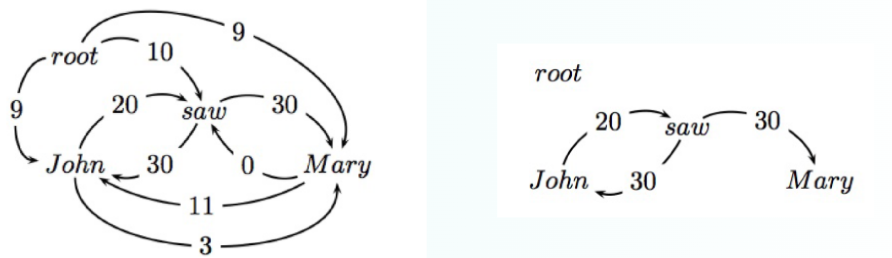
\includegraphics[scale=0.33]{45.png}
\end{center}
Another solution is the \textbf{Chu-Liu-Edmonds}: if it's not a tree, identify cycle and contract. Then recalculate arc weights in and out of the cycle. $O(n^2)$ complexity for non-projective trees (much slower than transition-based parsers).
\paragraph{NN Graph-Based Parser} Revived graph-based dependency parsing in a neural world, with great results although slower than neural dependency-based parsers.\\
Bidirectional LSTMs over word/tag embeddings.
\begin{center}
	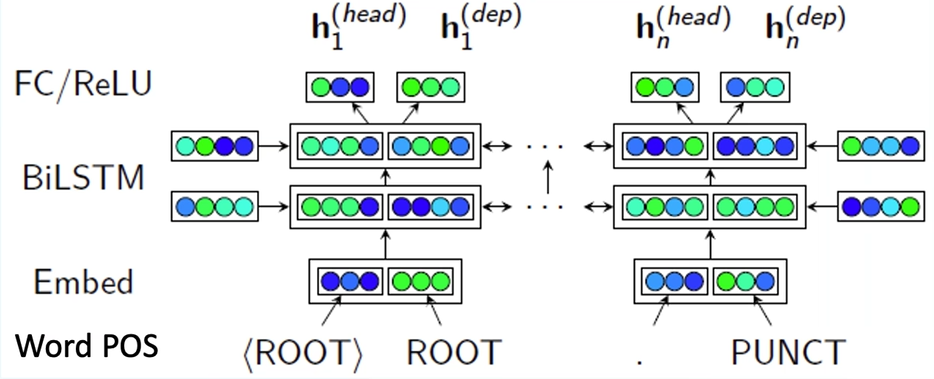
\includegraphics[scale=0.5]{38.png}
\end{center}
\subparagraph{Parser} Two separate FC ReLU (Fully Connected Rectified Linear Units) layers:
\begin{list}{}{}
	\item One representing each token as a dependent trying to find its head.
	\item One representing each token as a head trying to find its dependents.
\end{list}
\subparagraph{Dependency Relations} Two separate FC ReLU layers:\begin{list}{}{}
	\item One representing each token as a dependent trying to determine its label.
	\item One representing each token as a head trying to determine its dependents labels.
\end{list}
\begin{center}
	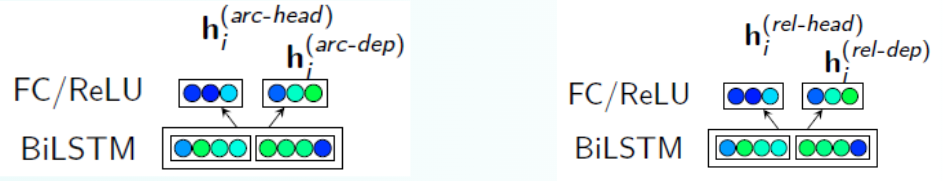
\includegraphics[scale=0.5]{46.png}
\end{center}
\subparagraph{Self-Attention} Biaffine self-attention layer to score a possible heads for each dependent.
A $n\times n$ matrix score:
\begin{center}
	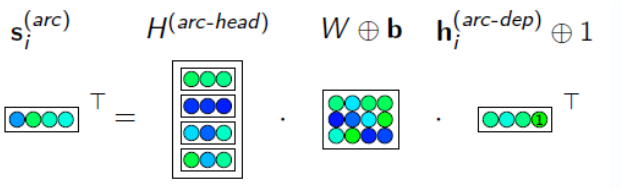
\includegraphics[scale=0.5]{47.png}
\end{center}
$$s_i = H^{\hbox{(arc-head)}}\cdot\left(Wh_i^{\hbox{(arc-dep)}}+b\right)$$
$$H^{\hbox{(arc-head)}} = \left[h_1^{\hbox{(arc-head)}}\:\ldots\:h_n^{\hbox{(arc-head)}}\right]$$
Train with cross-entropy and apply a spanning tree algorithm at inference time.
\subparagraph{Classifier for Labels} Biaffine layer to score possible relations for each best-head/dependent pair, $n\times c$
\begin{center}
	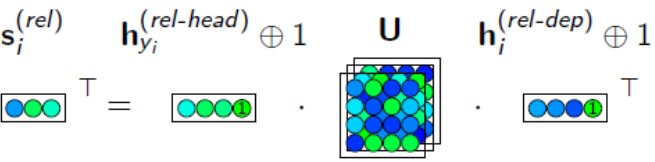
\includegraphics[scale=0.5]{48.png}
\end{center}
Train with softmax cross-entropy, added to the loss of the unlabeled parser.
\section{Universal Dependencies}
Treebank annotation schemes vary across languages, hard to compare results across them. Also hard to use to build multilingual.
\begin{center}
	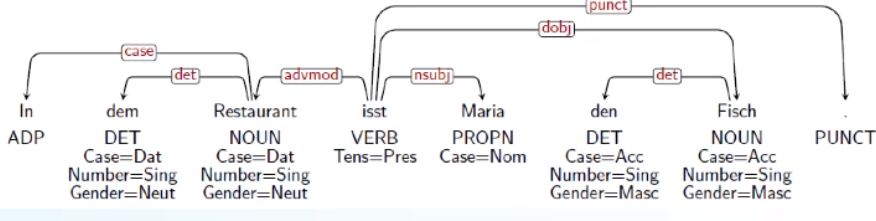
\includegraphics[scale=0.5]{39.png}
\end{center}
\paragraph{Goal} Facilitate consistent notation of similar constructions across languages. Support multilingual NLP and linguistic research. Build on common usage and existing de-facto standards. Complement and not replace language-specific schemes. \textbf{Community effort}.
\paragraph{Guiding Principles} Allow parallelism across languages:
\begin{list}{}{}
	\item Don't annotate same thing in different ways
	\item Don't make different things look the same
	\item Don't annotate things that are not there
	\item Use a universal pool of categories
\end{list}
Allows language-specific axioms.
\paragraph{Design Principles}\begin{list}{}{}
	\item \textbf{Dependency}: widely used in practical NLP systems, available in treebanks for many languages.
	\item \textbf{Lexicalism}: the basic annotation units are syntactic words, they have morphological properties and can enter into syntactic relations.
	\item \textbf{Recoverability}: transparent mapping from input text to word segmentation.
\end{list}
\paragraph{Morphological Annotation} 
\begin{center}
	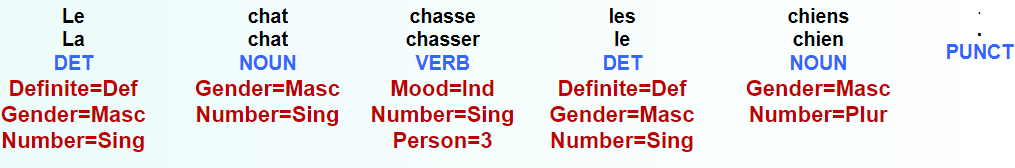
\includegraphics[scale=0.5]{49.png}
\end{center}
\begin{list}{}{}
	\item \textbf{Lemma} represent the semantic content of a word
	\item \textbf{Part-of-Speech} tag represent its grammatical class
	\item \textbf{Morphological Features} represent lexical and grammatical properties of the lemma or the specific word form
\end{list}
\paragraph{Syntactic Annotation}
\begin{center}
	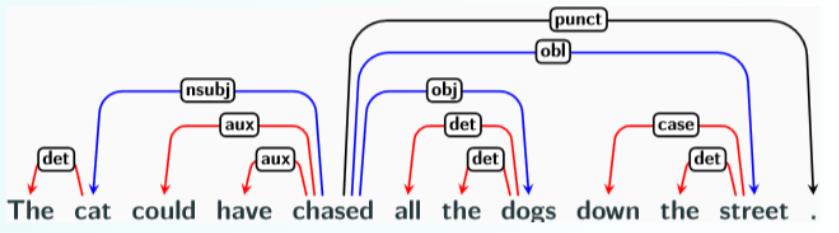
\includegraphics[scale=0.5]{50.png}
\end{center}
\begin{list}{}{}
	\item \textbf{Content Words} are used as heads of dependency relations
	\item \textbf{Function Words} attach to the content word they modify
	\item \textbf{Punctuation} attach to the head of phrase or clause
\end{list}
\paragraph{Coordination} The first conjunct is the head of all following conjuncts.
\begin{center}
	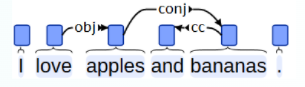
\includegraphics[scale=0.6]{51.png}
\end{center}
Attach coordinating conjunctions and punctuation to the immediately succeeding conjunct.
\begin{center}
	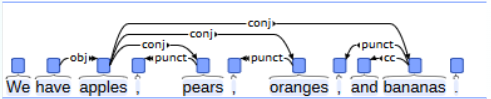
\includegraphics[scale=0.5]{52.png}
\end{center}
Except for the right headed constructions.
\begin{center}
	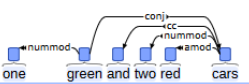
\includegraphics[scale=0.75]{53.png}
\end{center}
\paragraph{Enhanced Dependencies} Making some of the implicit relations between words more explicit, to facilitate relation extractions
\begin{list}{}{}
	\item Propagation of conjuncts
	\begin{center}
		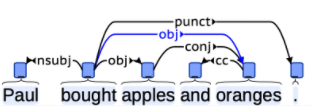
\includegraphics[scale=0.5]{54.png}
	\end{center}
	\item Conjoined verb and phrases
	\begin{center}
		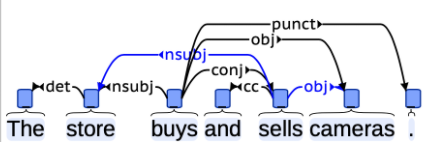
\includegraphics[scale=0.5]{55.png}
	\end{center}
	\item Subject from controller phrases
	\begin{center}
		\includegraphics[scale=0.5]{56.png}
	\end{center}
\end{list}
\begin{multicols}{2}
\paragraph{Basic}
\begin{center}
	\includegraphics[scale=0.5]{57.png}\\
	\includegraphics[scale=0.5]{58.png}
\end{center}
\paragraph{Enhanced}
\begin{center}
	\includegraphics[scale=0.5]{59.png}\\
	\includegraphics[scale=0.5]{60.png}
\end{center}
\end{multicols}
\pagebreak
\paragraph{Dependency Structure} The same concept expressed in different languages is represented in similar ways.
\begin{center}
	\includegraphics[scale=0.5]{40.png}
\end{center}
Keeping the content words as heads promotes parallelism across languages. The main grammatical relations involving a passive verb, a nominal subject and an oblique agent are the same.
\paragraph{Parsing}
Can train a parser, also possible to train on multiple languages.
\section{Machine Translation}
Main task that let to the creation of the field. MT is translating a text from one language to another.
\paragraph{Issues}
\begin{list}{}{}
	\item Sentence segmentation (e.g. 4 English sentences to 1 Chinese sentence)
	\item Grammatical differences
	\item Stylistic and cultural differences 
\end{list}
\paragraph{Alignment}
\begin{center}
	\includegraphics[scale=0.5]{61.png}
\end{center}
Not just literature! For example, in the European Parliament there are more official languages so all official documents have to be produced in all official languages.
\paragraph{MT Already Good for...}\begin{list}{}{}
	\item Tasks for which a rough translation is fine: extracting informations, web pages, email\ldots
	\item Tasks for which the MT can be post-edited: MT as first-pass, computer-aided human translation\ldots
	\item Tasks in sublanguage domain where high-quality MT is possible: FAHQT (Fully Automatic High Quality Translation)
\end{list}
\paragraph{MT Not Yet Good Enough for...}\begin{list}{}{}
	\item Really hard stuff: literature, natural spoken speech\ldots
	\item Really important stuff: medical translations in hospitals, emergency phone calls\ldots
\end{list}
\subsection{Language Similarities and Divergences}
Some aspects of human language are universal or near-universal, others diverge greatly.
\paragraph{Typology} Systematic study of these similarities and divergences. What are the dimension along which human languages vary?
\paragraph{Morphology}
\begin{list}{}{}
	\item \textbf{Morpheme}: minimal meaningful unit of language.
	\item \textbf{Word}: Morpheme + Morpheme + \ldots
	\item \textbf{Stems} root plus derivational morphemes\\
	\textbf{Hope}+ing $\Rightarrow$ \textbf{hop}ing
	\textbf{Lemma}: also called base form, root, lexeme\\
	\textbf{Hoping} $\Rightarrow$ \textbf{Hope}
	\textbf{Affixes}: \begin{list}{}{}
		\item Prefixes
		\item Suffixes
		\item Infixes
		\item Circumfixes
	\end{list}
\end{list}
\paragraph{Morphological Variation}
In isolating languages a single word generally have one morpheme, while in polysynthetic languages single words can have many morphemes.\\
In agglunative languages morphemes have clean boundaries, in fusion languages a single affix can have many morphemes.\\\\
So there's a wide range of synthesis: from vietnamese (isolating) to english to russian to onedia (synthetic).\\
The other range is fusion: from swahili (agglunative) to russian and oneida (fusion).
\paragraph{Segmentation Variation} Not every writing system has word boundaries marked between words, also some languages have very long sentences.\\
Some cold languages require the hearer to do more "figuring out", while in hot languages for example the subject of the sentence is always required.
\paragraph{Lexical Gaps} For example, Japanese doesn't have a word for "privacy", or English lacks the word for the Japanese "Oyakoko".
\paragraph{Event-To-Argument Divergences} In verb-framed languages we mark the direction of motion on verb, while in satellite-framed languaged we mark the direction in the satellite.
\subsection{Classical Techniques} Three classical ones:\begin{list}{}{}
	\item Direct
	\item Transfer
	\item Interlingua
\end{list}
\begin{center}
	\includegraphics[scale=0.75]{41.png}
\end{center}
\paragraph{Direct Translation} Proceed word-by-word in the text translating each, without intermediate structures except morphology. Knowledge is in the form of a huge bilingual dictionary and some word-to-word translation information.\\
The dictionary can be more specific for each word, specifying cases and different translation for each case.\\
The main problem is that we don't "translate" the different syntactic structures and maintain the order of the words of the original language which is often different in the target language.
\subparagraph{Pros} Fast, simple, cheap, no translation rules hidden in the lexicon.
\subparagraph{Cons} Unreliable, not powerful, rule proliferation, need major restructuring after lexical subsitution.
\paragraph{Transfer Model} We use a set of \textbf{transfer rules} that restructure the parse tree. But we need hard to obtain lexical transfer rules. We apply contrastive knowledge: knowledge about the difference between two languages.
\begin{list}{}{}
	\item \textbf{Analysis}: syntactically parse source language
	\item \textbf{Transfer}: rules to turn this parse into parse tree for target language
	\item \textbf{Generation}: generate target sentence from parse tree
\end{list}
\subparagraph{Lexical Transfer} Transfer-based systems also need lexical transfer rules, bilingual dictionaries. Can be a list or a word disambiguation system.
\subparagraph{Systram} Combination of direct and transfer.\begin{list}{}{}
	\item Analysis:\begin{list}{}{}
		\item Morphological analysis, POS tagging
		\item Chunking of NPs, PPs, phrases
		\item Shallow dependency parsing
	\end{list}
	\item Transfer:\begin{list}{}{}
		\item Translation of idioms
		\item Word sense disambiguation
		\item Assigning prepositions based on governing verbs
	\end{list}
	\item Synthesis:\begin{list}{}{}
		\item Apply rich bilingual dictionary
		\item Deal with reordering
		\item Morphological generation
	\end{list}
\end{list}
$N^2$ set of transfer rules, grammar and lexicon full of language-specific stuff, hard to build and maintain.
\paragraph{Interlingua} Instead of language-to-language rules, we abstract the meaning of the sentence and translate that.\begin{enumerate}
	\item Translate source sentence into meaning representation
	\item \textbf{Generate} target sentence from meaning
\end{enumerate}
\begin{center}
	\includegraphics[scale=0.5]{62.png}
\end{center}
The idea is that some of the MT work that we need to do is part of other NLP tasks: disambiguating eng:book-ita:libro from eng:book-ita:prenotare. So we could have concepts like BOOKVOLUME and PRENOTARE and solve this problem once for each language.
\subparagraph{Pros} Avoids the $N^2$ problem, and easier to write rules.
\subparagraph{Cons} Semantics is hard, useful information lost (because we paraphrase).

\subsection{Statistical Machine Translation}
\paragraph{Example} Start from a parallel corpus: a set of sentences in a language and the corresponding sentences in the other language.\\
Have a sentence to translate into an unknown target sentence into the target language. For each word in the sentence, look for that into the parallel corpus, trying to figure out the translation. 	
\paragraph{What Makes a Good Translation} Two facts to maximize:
\begin{list}{}{}
	\item \textbf{Faithfulness} or fidelity: how close is the meaning of the translation to the meaning of the original.\\
	Even better: does the translation cause the reader to draw the same inferences as the original would have?
	\item \textbf{Fluency} or naturalness: how natural the translation is, just considering its fluency in the target language.
\end{list}
Faithfulness and fluency are formalized: best-translation $\hat{T}$ of a source sentence S
$$\hat{T}=\arg\max_T \left\{\hbox{Fluency}(T)\cdot\hbox{Faithfulness}(T,S)\right\}$$
Called the \textbf{IBM model}. It's the Bayes rule
$$\hat{T} = \arg\max_T P(T)P(S\:|\:T)$$
More formally: assume we want to translate from a foreign language sentence $F$ to an English language sentence $E$
$$F = f_1 \ldots f_m$$
We want to find the best English sentence
$$\overline{E} = e_1\ldots e_n = \arg\max_E P(F\:|\:E)P(E)$$
With $P(E)$ from the language model and $P(F\:|\:E)$ from the translation model.\\
Also known as noisy model
\begin{center}
	\includegraphics[scale=0.5]{42.png}
\end{center}
\paragraph{Fluency $P(T)$} How to measure that a sentence is more fluent than another? E.g. "That car was almost crash onto me" is less fluent than "That car almost hit me".\\
The answer is language models, $n$-grams! For example, $P($hit$\:|\:$almost$)>P($was$\:|\:$almost$)$.\\
But can use any other more sophisticated model of grammar. Advantage: it's monolingual knowledge.
\paragraph{Faithfulness $P(S\:|\:T)$} How to quantify? Intuition: degree to which words in one sentence are plausible translations of words in the other sentence. Product of probabilities that each word in target sentence would generate each word in source sentence.\\
Need to know, for every target language word, probability of it mapping to every source language word. How to learn this? Parallel texts: lots of times we have two texts that are translations of each other. If we knew which word in Source text mapped to each word in Target text, we could just count.
\subparagraph{Sentence Alignment} Figuring out which source language sentence maps to which target language sentence.
\subparagraph{Word Alignment} Figuring out which source language word maps to which target language word. \\\\
The faithfulness model $P(S\:|\:T)$ just models a "bag of words" which words come from e.g. English to Italian.\\
$P(S\:|\:T)$ doesn't have to worry about internal facts about target word order, that's the job of $P(T)$.\\
$P(T)$ can do bag generation: put the following words in order.
\paragraph{Three Problems for Statistical Machine Translation}
\begin{list}{}{}
	\item \textbf{Language Model}: given an English string $e$, assigns $P(e)$ by a formula such that:
	\begin{list}{}{}
		\item Good English string $\Rightarrow$ high $P(e)$
		\item Random word sequence $\Rightarrow$ low $P(e)$
	\end{list}
	Can be trained on large, unsupervised mono-lingual corpus for the target language, and could use more sophisticated PCFG language model to caputre long-distance dependencies. Terabytes of web data used to build large 5-gram models.
	\item \textbf{Translation Model}: given a pair of strings $\langle f,e\rangle$, assigns $P(f\:|\:e)$ by a formula such that:
	\begin{list}{}{}
		\item $\langle f,e\rangle$ look like translations $\Rightarrow$ high $P(f\:|\:e)$
		\item $\langle f,e\rangle$ don't look like translations $\Rightarrow$ low $P(f\:|\:e)$
	\end{list}
	\item \textbf{Decoding Algorithm}: given a language model, a translation model and a new sentence $f$, it finds the translation $e$ that maximize $P(e)P(f\:|\:e)$
\end{list}
\subsection{Phrase Based Machine Translation}
Follows three steps
\begin{enumerate}
	\item Group words into phrases
	\item Translate each phrase
	\item Move the phrases around
\end{enumerate}
$P(F\:|\:E)$ is modeled by translating phrases in $E$ to phrases in $F$. First segment $E$ into a sequence of phrases $\overline{e}_1,\ldots,\overline{e}_I$, then translate each $\overline{e}_i$ into $\overline{f}_i$ based on \textbf{translation probability} $\phi(\overline{f}_i\:|\:\overline{e}_i)$. Then, reorder translated phrases based on \textbf{distortion probability} $d(i)$ for the $i$the phrase.
\paragraph{Translation Probabilities} Assuming a phrase aligned parallel corpus is available or constructed that show matching between phrases in $E$ and $F$. Then compute (MLE) estimate of $\phi$ based on simple frequency counts $$\phi(\overline{f},\overline{e})=\frac{\hbox{Count}(\overline{f},\overline{e})}{\sum_{f} \hbox{Count}(f,\overline{e})}$$
\paragraph{Distortion probability} The probability that a phrase in position $X$ in the original sentence moves to position $Y$ in the translation.\\
Distortion is the measure of distance between positions of corresponding phrases in the 2 languages. Distortion of phrase $i$ as the distance between the start of the foreign phrase generated by $\overline{e}_i$ ($a_i$ and the end of the foreign phrase generated bu the previous phrase $\overline{e}_{i-1}$ ($b_{i-1}$). Typically we assume the probability of a distortion decreases exponentially with the distance of the movement $$d(i) = c\alpha^{|a_i-b_{i-1}|}$$
Set $0<\alpha<1$ base on fit to phrase-aligned training data. Then set $c$ to normalize $d(i)$ so that it sums to 1.
\paragraph{Training $P(F\:|\:E)$} What we mainly need to train is $\phi(f_j\:|\:e_i)$\\
Suppose we had a large bilingual training corpus: a \textbf{bitext}. Suppose also to know exactly which phrase in the target language was the tranlsation of which phrase in the source language: \textbf{phrase alignment}.\\
If we had this, we could just count-and-divide
$$\phi(\overline{f},\overline{e})=\frac{\hbox{Count}(\overline{f},\overline{e})}{\sum_{f} \hbox{Count}(f,\overline{e})}$$
But we don't have phrase alignments. We have \textbf{word alignments}.
\begin{center}
	\includegraphics[scale=0.5]{43.png}
\end{center}
Actually we have more restrictive word alignments. Word alignments are mapping between source and target words in parallel sentence. Restriction: each foreign word come from exactly one source word.
\begin{center}
	\includegraphics[scale=0.5]{44.png}
\end{center}
Advantage: represent alignment by the index of the English word that the french word comes from. The above alignment thus is 2,3,4,5,6,6,6.\\
\textbf{Spurious words} are words in the foreign sentence that does not align with any word in the source language. We assume one to many alignment: each word in $F$ aligns with 1 word in $E$, with some words in $F$ coming from NULL.
\paragraph{Computing Word Alignments} IBM-Model 1. For phrase-based machine translation we need a word-alignment to extract a set of phrases.\\
A word alignment model gives us $P(F,E)$, and we want this to train our phrase probabilities $\phi(f_j\:|\:e_j)$ as part of $P(F\:|\:E)$.\\
A word-alignment model allows to compute the translation probability $P(F\:|\:E)$ by summing the probabilities of all possible $(l+1)^m$ "hidden" alignments $A$ between $F$ and $E$
$$P(F\:|\:E) = \sum_A P(F, A\:|\:E)$$
IBM-Model 1 assumes the following simple generative model of producing $F$ from $E=e_1,\ldots,e_l$:
\begin{enumerate}
	\item Choose length $J$ of $F$ sentence: $F=f_1,\ldots,f_J$
	\item Choose a 1 to many alignment $A=a_1,\ldots,a_J$
	\item For each position $j$ in $F$, \textbf{generate} a word $f_j$ from the aligned word $e_{a_j}$ in $E$
\end{enumerate}
Its goal is to find the most probable alignment given a prameterized model
$$\hat{A}=\arg\max_A P(F,A\:|\:E) = \arg\max_A\prod_{j=1}^J t(f_j,e_{a_j})$$
Since translation choice for each position $j$ is independent, the product is maximized by maximizing each term
$$a_j = \arg\max_{0\leq i\leq l} t(f_j,e_i)\:\:\:\:\:1\leq j\leq l$$
\paragraph{Training Alignment Probabilities}\begin{list}{}{}
	\item Get a parallel corpus, e.g.: Europarl, Hansards\ldots
	\item Sentence alignment. Intuition: use length in words or chars, together with dynamic programming. Ora a simpler MT model.
	\item Use Expectation Maximization to train word alignments.\\
	We can bootstrap alignment from a sentence-aligned bilingual corpus using the EM algorithm.\\
	$P(A\:|\:E,F)$ is the probability of the alignment $A$ given a translated pair of sentences $E$ and $F$
	$$P(A\:|\:E,F) = \frac{P(F,A\:|\:E)}{P(F\:|\:E)} =\frac{P(F,A\:|\:E)}{\sum_{A'}P(F,A'\:|\:E)}$$
	Inherent hidden structure is revealed by EM training.
\end{list}
\subparagraph{EM Algorithm for Word Alignment}\begin{lstlisting}
Randomly set model parameters, making sure they represent legal distributions
Until convergence (i.e. parameter no longer change) do:
	E Step: compute the probability of all possible alignments
		of the training data using the current model
	M Step: use these alignment probability estimates to re-estimate values
		for all of the parameters
end
\end{lstlisting}
\subsubsection{Phrase-Based Translation Model}
Major components of a phrase-based model:
\begin{list}{}{}
	\item Phrase translation model $\phi(f\:|\:e)$
	\item Reordering model $\Omega(f\:|\:e)$
	\item Language model $P_{LM}(e)$
\end{list}
Bayes rule
$$\arg\max_e P(e\:|\:f) = \arg\max_e P(f\:|\:e)P(e) = \arg\max_e\phi(f\:|\:e)P_{LM}(e)\Omega(f\:|\:e)$$
Sentences $f$ and $e$ are decomposed into $I$ phrases: $\overline{f}_1^I = \overline{f}_1,\ldots,\overline{f}_I$
$$\phi(f\:|\:e)=\prod_{i=1}^I\phi(\overline{f}_1,\overline{e}_i)d(a_i-b_{i-1})$$
\paragraph{Phrase Alignment} Alignment algorithms produce one-to-many word translations, and we know that words do not map one-to-one in translations. Better to map "phrases", sequences of words, to phrases and probabilistically reorder them in translation.\\
Combine $E\rightarrow F$ and $F\rightarrow E$ word alignments to produce a phrase alignment.
\paragraph{Decoding}
\paragraph{Evaluation} Human subjective evaluation is best but time consuming and expensive. Automated evaluation comparing the output to multiple human reference translations is cheaper and correlates with human judgments.\\
Better: computer-aided translation evaluation. \textbf{Edit cost}: measure the number of changes that a human translator must make to correct the MT output (number of words changed, amount of time taken, number of keystrokes\ldots).
\subparagraph{Scores} Based on similarity to the reference translations:
\begin{list}{}{}
	\item \textbf{BLEU} (Bilingual Evaluation Understudy): determine the number of $n$-grams of various sizes that the MT output shares with the reference translations. Compute a modified precision measure of the $n$-grams in MT result, averaging $n$-gram precision over all $n$-grams up to size $N$ (typically 4) using the geometric mean:
	$$p_n = \frac{\sum_{C\in\hbox{Corpus}}\sum_{n\hbox{-gram}\in C}\hbox{Count}_{\hbox{clip}}(n\hbox{-gram})}{\sum_{C\in\hbox{Corpus}}\sum_{n\hbox{-gram}\in C}\hbox{Count}(n\hbox{-gram})}$$
	$$p = \sqrt[N]{\prod_{n=1}^Np_n}$$
	\textbf{BP} (Brevity Penalty): uses a penalty for the translations that are shorter than the reference translation. Define the effective reference length $r$ for each sentence as the length of the reference sentence with the largest number of $N$-gram matches. With $c$ the candidate sentence length:
	$$BP = \left\{\begin{array}{l l}
	1&c > r\\
	e^{\frac{1-r}{c}}& c\leq r
	\end{array}\right.$$
	The final BLEU score is 
	$$BLEU = BP\cdot p$$
	Correlates with human evaluation when comparing outputs from different SMT systems, but doesn't correlate with human judgments when comparing SMT systems with manually developed MT or MT with human translations.
\end{list}
\subsection{Syntax Based Statistical Machine Translation} SMT methods that adopt a syntactic transfer approach. Improved results demonstrated for translating between more distant language pairs (e.g. English-Chinese).
\paragraph{Synchronous Grammar} Multiple parse trees in a single derivation. Describes the hierarchical structures of a sentence and its translation, and also the correspondence between their sub-parts.
\begin{center}
	\includegraphics[scale=0.5]{94.png}
\end{center}
\paragraph{Synchronous Derivations and Translation Models} Need to make a probabilistic version of synchronous grammars to create a translation model for $P(F\:|\:E)$. Each synchronous production rule is given a weight $\lambda_i$, that is used in a maximum-entropy (log linear) model. Parameters are learned to maximize the conditional log-likelihood of the training data
$$\lambda^* = \arg\max_\lambda\sum_j\log P_\lambda(f_j\:|\:e_j)$$
\paragraph{Use of Dependency Parsing} Restrict phrases to those corresponding to parse subtrees, and use the parse trees to learn reordering of source language to make it more similar to target language and train a PBMT system on the rearranged parallel corpus.
\subsection{Minimum Error Rate Training} Also known as MERT. No longer using the noisy channel model, but MERT: train a \textbf{logistic regression classifier} to directly minimize the final evaluation metric on the training corpus by using various features of a translation
\begin{list}{}{}
	\item Language model $P(E)$
	\item Translation model $P(F\:|\:E)$
	\item Reverse translation model $P(E\:|\:F)$
\end{list}
\paragraph{Conclusions} Statistical PBMT: phrase table derived by symmetrizing word alignments on a sentence-aligned parallel corpus, statistical phrase translation model $P(F\:|\:E)$ and language model $P(E)$.\\
All these combined in a logistic regression classifier trained to minimize error rate.
\section{Neural Machine Translation}
Statistical Machine Translation is a huge research field, but requires the compilation and maintainment of extra resources (for example tables of equivalent phrases), thus lots of human effort to maintain.\\
In 2014 neural machine translation was introduced with an huge impact on the machine translation field.
\paragraph{NMT} Neural Machine Translation is a way of doing MT with a \textbf{single neural network}, a sequence-to-sequence (seq2seq) one.\begin{center}
	\includegraphics[scale=0.6]{63.png}
\end{center}
A seq2seq model is versatile: a neural network takes an input an produces a neural representation, which is used as input by a second network that produces a sequence as output. These models are useful for more than just MT, many natural language processing tasks can be phrased as sequence-to-sequence:
\begin{list}{}{}
	\item Summarization, long text to short text.
	\item Dialogue, previous utterances to next utterance
	\item Parsing, input text to sequence of parsing symbols
	\item Code generation, natural language to e.g. Python code
\end{list}
The seq2seq model is an example of \textbf{conditional language model}:\begin{list}{}{}
	\item \textbf{Language model} because the decoder is predicting the next word of the target sentence $y$
	\item \textbf{Conditional} because its predictions are also conditioned on the source sentence $x$
\end{list}
NMT directly calculates $$P(y\:|\:x) = P(y_1\:|\:x)P(y_2\:|\:y_1,x)\ldots P(y_T\:|\:y_1,\ldots,y_{T-1},x)$$
To train a NMT system, get a big parallel corpus\ldots
\begin{center}
	\includegraphics[scale=0.6]{64.png}
\end{center}
\paragraph{Beam Search} We showed how to generate (decode) the target sentence by taking the argmax on each step of the decoder. But this is greedy decoding, taking the most probable word on each step, but it has problems e.g. it has no way to undo decisions! A better option would be to use \textbf{beam search}, to explore several hypothesis and select the best one. Ideally we want to find a translation $y$ that maximizes $$P(y\:|\:x) = \prod_{i=1}^T P(y_i\:|\:y_1,\ldots,y_{i-1},x)$$
We could try computing all possible sequences $y$: on each step $t$ of the decoder we're tracking $V^t$ possible partial translations with $V$ vocab size. This $O(V^T)$ complexity is too expensive, though, so \textbf{beam search}: we keep track of the $k$ most probable partial translations, with $k$ being the beam size ($k\simeq 5, 10$ in practice).\\
An hypothesis has a score which is its log probability $$\hbox{score}(y_1,\ldots,y_t) = \sum_{i=1}^t \log P_{LM}(y_i\:|\:y_1,\ldots,y_{i-1},x)$$
Scores are all negative, the higher the better. We search for high-scoring hypothesis, tracking top $k$ on each step.\\
Doesn't guarantee to find the most optimal solution, but it's far more efficient.
\subparagraph{Example} With $k=2$
\begin{center}
	\includegraphics[scale=0.6]{65.png}
\end{center}
Then we go back finding the complete translations.
\subparagraph{Stopping Criterion} In greedy decoding, we decode until we find the END token. In beam search, different hypothesis can produce the END tokens on different timesteps: we place it aside and continue exploring other hypothesis. Usually we continue beam search until:\begin{list}{}{}
	\item we reach a timestep $T$, a predefined cut-off, or
	\item we have at least $n$ completed hypothesis, another predefined cut-off
\end{list}
\subparagraph{Finishing Up} When we have the list of hypothesis, how we select the highest scoring one? Each hypothesis has its score, but longer hypothesis have lower scores so we normalize by length
$$\hbox{score}(y_1,\ldots,y_t) =\frac{1}{t}\sum_{i=1}^t \log P_{LM}(y_i\:|\:y_1,\ldots,y_{i-1},x)$$
\begin{multicols}{2}
\subparagraph{Benefits}\begin{list}{}{}
	\item Better Performance: more fluent, better use of context and of phrase similarities
	\item Single neural network to be optimized end-to-end: no subcomponents to be individually optimized
	\item Requires much less human engineering effort: no feature engineering, same method for all language pairs.
\end{list}
\columnbreak
\subparagraph{Disadvantages}\begin{list}{}{}
	\item NMT is less interpretable and hard to debug
	\item NMT is difficult to control: can't easily specify rules or guidelines for translations, also safety concerns
\end{list}
\end{multicols}
\textbf{Machine translation is not a solved problem}, many difficulties remain:
\begin{list}{}{}
	\item out-of-vocabulary words
	\item domain mismatch between train and test data
	\item maintaining context over longer texts
	\item failures to accurately capture sentence meaning
	\item pronouns (or zero pronoun) resolution errors
	\item morphological agreement errors
	\item low-resource language pair
\end{list}
NMT is the flagship task for NLP deep learning: it has pioneered many of the recent innovations of NLP. In 2021 NMT research continues to thrive, researchers have found many improvements to the vanilla seq2seq NMT system presented thus far. But one improvement is so integral that is has become the new vanilla.
\paragraph{Attention} Seq2seq has a bottleneck: the encoding needs to capture all the information about the source sentence, it's an \textbf{information bottleneck}.\\
\textbf{Attention} provides a solution to the bottleneck problem. The core idea is: on each step of the decoder, focus on a particular part of the source sequence.
\begin{center}
	\includegraphics[scale=0.6]{67.png}
\end{center}
\subparagraph{In equations}\begin{list}{}{}
	\item We have the hidden states in the encoder $h_1,\ldots,h_N\in R^h$
	\item On timestep $t$ we have the decoded hidden state $s_t \in R^h$
	\item We get the attention scores $e^t$ for this step 
	$$e^t=[s_t^Th_1,\ldots,s_t^Th_N]\in R^N$$
	\item We take the softmax to get the attention distribution for this step (probability distribution that sums to 1)
	$$\alpha^t=\hbox{Softmax}(e^t) \in R^N$$
	\item We use $\alpha^t$ to take a weighted sum of the encoder hidden states to get the attention output $a^t$
	$$a^t = \sum_{i=1}^N \alpha_i^th_i\in R^h$$
	\item Finally, we concatenate the attention output with the decoder hidden state and proceed as in the non-attention seq2seq model
	$$[a_t, s_t]\in R^{2h}$$
\end{list}
Attention significantly improves NMT performance, solving the bottleneck problem and helping with vanishing gradient problem. Also provides some interpretability, and we get alignment for free: we never explicitly trained an alignment system, the network just learned alignment by itself.
\subparagraph{Attention Variants} We have some values $h_i\in R^h$ and a query $s\in R^h$. Attention involves:
\begin{list}{}{}
	\item Computing the attention scores $e\in R^N$
	\item Taking softmax to get a attention distribution
	$$\alpha=\hbox{Softmax}(e) \in R^NJ$$
	\item Using $\alpha$ to take the weighted sum of values
	$$\alpha = \sum_{i=1}^N\alpha_ih_i\in R^h$$
	Thus obtaining the \textbf{attention output} $\alpha$ (sometimes called the \textbf{context vector})
\end{list}
We've seen it in translation, but this can be applied to other NLP tasks. It has becomes a general deep learning technique as well.\\
A more general definition of attention is: given a set of vector values, and a vector query, attention is a technique to compute a weighted sum of the values dependent on the query. We sometimes say that the query \textit{attends to} the values. E.g. in the seq2seq + attention model, each decoder hidden state (query) \textit{attends to} all the encoder hidden states (values).\\
\textbf{Attention is all you need}. Self-attention helps to contextualize words: a limit on word embeddings was that each word had a single vector, with attention we can introduce into the representation the context into which they appears, allowing to observe other words.
%skip until Google neural MT architecture
\subsection{Self-Attention}
Sequence to sequence models with attention are quite effective in transduction tasks, but their sequential nature limits parallelism. The \textbf{transformer} transduction model relies entirely on self-attention to compute representations of its input and output: it doesn't use sequence aligned RNNs nor convolutions.\\
As a result, training costs are reduced by 1-2 orders of magnitude.\\\\
So we want \textbf{parallelization} but RNNs are inherently sequential. They also generally need attention mechanism to deal with long range dependencies: path length between states grows with distance otherwise. We may be able to just use attention and skip the need for the RNN.
\paragraph{Attention} Given a set of vector values and a vector query, attention is a technique to compute a weighted sum of the values dependent on the query.\\
The intuition is the following: the weighted sum is a selective summary of the information contained in the values, where the query determines which values to focus on. Attention is a way to obtain a fixed-size representation of an arbitrary set of representations (the values), dependent on some other representation (the query).\\\\
The generic attention, as we have seen before: we have some \textbf{values} $v_1,\ldots,v_N\in R^{d_1}$, some \textbf{keys} $k_1,\ldots,k_N\in R^{d_1}$ and a \textbf{query} $s\in R^{d_2}$\begin{list}{}{}
	\item Compute the \textbf{attention scores} $e\in R^N$
	\item Taking softmax to get the \textbf{attention distribution} $\alpha=\hbox{Softmax}(e)\in R^N$
	\item Using the attention distribution to take the weighted sum of values $$a = \sum_{i=1}^N\alpha_iv_i\in R^{d_1}$$
	Thus obtaining the \textbf{attention output} or context vector $a$
\end{list}
There are variants, several ways to compute $e\in R^{d_1}$:
\begin{list}{}{}
	\item Basic dot-product attention $e_i=s^Tk_i\in R$\\
	This assumes $d_1=d_2$, and is the version used in NMT
	\item Multiplicative attention $e_i=s^TWk_i\in R$\\
	Where $W\in R^{d_1\times d_2}$ is a weight matrix
	\item Additive attention $e_i=w^T\tanh(W_1k_1+W_2s)\in R$\\
	Where $W_1\in R^{d_3\times d_1}$, $W_2\in R^{d_3\times d_2}$ are weight matrices and $w\in R^{d_3}$ is a weight vector.\\$d_3$ is the attention dimensionality, hyperparameter.
\end{list}
\paragraph{Issues with Recurrent Models}\begin{list}{}{}
	\item O(sequence length) steps for distant word pairs to interact. This means: hard to learn long-distance dependencies (because gradient problems!) and linear order of words "baked in" (and we already know that linear order isn't the right way to think about sentences
	\item Non-parallelizable
\end{list}
What can we use instead of recurrence?
\paragraph{Word Windows} Word window models aggregate local contexts (also known as 1D convolution). Stacking window layers allow interaction between farther words. The maximum interaction distance is $\frac{\hbox{sequence length}}{\hbox{window size}}$
\paragraph{Attention} Attention treats each word's representation as a query to access and incorporates information from a set of values. We saw attention from decoder to encoder, let's see attention withing a single sentence. The maximum interaction distance becomes O(1) since all words interact at every layer!
\paragraph{Self-Attention}
We can think of attention as an approximated hashtable:
\begin{list}{}{}
	\item To look up a value we compare a query against keys in the table
	\item In a hashtable: each query (hash) maps to exactly one key-value pair
	\item In (self-)attention: each query matches each key to varying degrees. We return a sum of values weighted by the query-key match.
\end{list}
Given the \textbf{queries} $q_1,\ldots,q_T\in R^d$, the \textbf{keys} $k_1,\ldots,k_T\in R^d$ and the \textbf{values} $v_1,\ldots,v_T\in R^d$ (but in practice the number of queries can differ from the number of keys and values), in self-attention \textbf{the queries, keys and values are drawn from the same source}. E.g.: if the output of the previous layer is $x_1,\ldots,x_T$ (one vector per word), we could use $v_i=k_i=q_i=x_i$ (same vector for all of them).\\
The dot product self-attention operation is:
\begin{list}{}{}
	\item Compute key-query quantities $$e_{ij} = q_i^Tk_jk$$
	\item Compute attention weights from affinities $$\alpha_{ij}=\frac{e^{e_{ij}}}{\sum_k e^{e_{ik}}}$$
	\item Compute outputs as weighted sum of values $$\hbox{Output}_i=\sum_j\alpha_{ij}v_j$$
\end{list}
\paragraph{Vector Notation}
\begin{list}{}{}
	\item With embeddings stacked in $X$, compute queries, keys and values: $Q=XW^Q, K=XW^K, V=XW^V$
	\item Compute attention scores between queries and keys $E = QK^T$
	\item Take the softmax to normalize attention scores $A=$ Softmax$(E)$
	\item Take a weighted sum of values Output = $AV$
\end{list}
$$\hbox{Output}=\hbox{Softmax}(QK^T)V$$
\paragraph{Self-Attention as a NLP Building Block}
\begin{center}
	\includegraphics[scale=0.5]{68.png}
\end{center}
This shows a stack of self-attention blocks like we might stack LSTM layers. Self-attention though cannot be a drop-in replacement for recurrence, for it has few issues.
\subparagraph{No Notion of Order} Self-attention is an operation on sets, meaning it has no inherent notion of order. Self-attention doesn't know the order of its inputs.\\
We need to encode the order of the sentence in our keys, queries and values. Consider representing each sequence index as a vector: $p_i\in R^d$, for $i\in\{1,\ldots,T\}$ are position vectors. It's easy to incorporate this info into our self-attention block: just add the $p_i$ into our inputs. With $\tilde{v}_i, \tilde{q}_i, \tilde{k}_i$ our old values, queries and keys
$$v_i = \tilde{v}_i+p_i$$
$$q_i = \tilde{q}_i+p_i$$
$$k_i = \tilde{k}_i+p_i$$
The $p_i$ can be \textbf{sinusoidal position representations}: concatenate sinusoidal functions of varying periods. Periodicity indicates that maybe an "absolute position" isn't important, but it's not learnable. So the $p_i$ can be all learnable: learn a matrix $p\in R^{d\times T}$ and the $p_i$s are columns of that matrix. It's flexible, because each position gets to be learned to fit the data, but can't be used to extrapolate indexes outside $1,\ldots,T$.
\subparagraph{Adding Non-Linearities} Therea re no elementwise nonlinearieis in self-attention, so stacking more self-attention layers just re-averages value records. A simple fix: we add feed-forward network to post process each output vector:
\begin{center}
	\includegraphics[scale=0.5]{69.png}
\end{center}
$$m_i = \hbox{MLP}(\hbox{Output}_i) + b_2 = W_2\cdot\hbox{ReLU}(W_1\cdot\hbox{Output}_i + b_1)+b_2$$
\subparagraph{Future} We need to ensure we don't "look at the future" when predicting a sequence, like in machine translation or language modeling. To mask the future, we could change the set of keys and queries to include only past words but it's inefficient. To enable parallelization, we mask out attention to future words by setting attention scores to $-\infty$
$$e_{ij}=\left\{\begin{array}{l l}
q^Tk_j&j<i\\
-\infty&j\geq i
\end{array}\right.$$
\subsection{Transformers}
The encoder maps an input sequence of symbol representations $(x_1,\ldots,x_n)$ to a sequence of continuous representations $(z_1,\ldots,z_n)$ Given $z$, the decoder then generates an output sequence $(y_1,\ldots,y_m)$ of symbols one element at a time. At each step, the model is \textbf{auto-regressive}, consuming the previously generated symbols as additional input when generating the next.
\begin{center}
	\includegraphics[scale=0.5]{70.png} \includegraphics[scale=0.5]{71.png}
\end{center}
The encoding component is a stack of encoders, and the decoding component is a stack of decoders of the same number.
\paragraph{Self-Attention} The encoder's inputs first flow into a self-attention layer, that helps the encoder look at other words in the input sentence as it encodes a specific word. The outputs of the self-attention layer are fed to a feed-forward neural network: the exact same FFNN in independently applied to each position.\\
The decoder has both those layers, with an attention layer between them that helps the decoder focus on the relevant parts of the input sentence.
\begin{center}
	\includegraphics[scale=1]{72.png}
\end{center}
\paragraph{Multi-Headed Attention} With a simple self-attention there's only a way for a word to interact with others. We can expand the model ability to focus on different positions: multiple sets of query/key/value weight matrices, apply attention and then concatenate outputs and pipe through linear layer.
\begin{enumerate}
	\item From the input sentence
	\item We embed each word (\textbf{word embeddings})\\
	In all encoders other than the first we don't need the embedding, we directly use the output of the previous encoder.
	\item We split into $n$ heads and multiply with weight matrices
	\item Calculate attention using the resulting $Q$/$K$/$V$ matrices
	\item Concatenate the resulting $Z$ matrices, then multiply with weight matrix $W^O$ to produce the output layer.
\end{enumerate}
\paragraph{Training Tricks}
\begin{list}{}{}
	\item \textbf{Residual Connections}: deep networks are bad at learning the identity function. Therefore, directly passing "raw" embeddings to the next layer can be helpful
	$$x_l = F(x_{l-1} + x_{l-1}$$
	\item \textbf{Layer Normalization}: may be difficult to train the parameters of a given layer because its input from the layer beneath keeps shifting. Solution: reduce uninformative variation by normalizing to zero mean and std. dev. one within each layer
	$$x_l' = \frac{x_l - \mu_l}{\sigma_l + \epsilon}$$
	Helps models to train faster.
	\item \textbf{Scaled Dot Product Attention}: after layer normalization, the mean and variance of vector elements is 0 and 1, respectively. However the dot product still tends to take on extreme values, as its variance scales with dimensionality $d_k$. The updated self-attention equation is $$\hbox{Output} = \hbox{Softmax}\left(\frac{QK^t}{\sqrt{d_k}}\right)V$$
\end{list}
\begin{center}
	\includegraphics[scale=0.75]{73.png}
\end{center}
\subsubsection{Transformers Library}
\paragraph{Hugging Face Transformers} Installed with \texttt{pip install transformers}.\\
Typical pattern is to load a model, then initialize two objects:
\begin{list}{}{}
	\item Tokenizer\\
	Can use specific tokenizer for specific model
	\item Model, three types: encoders (e.g. BERT), decoders (e.g. GPT2), encoder-decoders
\end{list}
\subsubsection{Transformers Architectures}
From pretrained word embeddings: start with pretrained word embeddings with no context, and learn to incorporate context in an LSTM or transformer while training on the task.\\
Issues: the training data we have for out downstream task (like question answering) must be sufficient to teach all contextual aspects of language. Also most of the parameters in our network are randomly initialized.\\\\
In modern NLP we pretrain the whole model: all (or almost all) NLP networks are initialized via pretraining. Pretraining methods hide parts of the inputs from the model, and then train the model to reconstruct those parts.\\This has been effective at building strong representations of language, parameter initialization for strong NLP models and probability distributions over language that we can sample from.
\paragraph{Pretraining Transformers} Two-step development\begin{center}
	\includegraphics[scale=0.5]{74.png}
\end{center}
\subparagraph{Pretraining through language modeling} Recall the language modelling task: model $P_\theta(w_t\:|\:w_{1:t-1})$, the probability distributions over words given their past contexts (lots of data for this).\\Pretraining through language modeling is training a neural network to perform language modeling on a large amount of texts and \textbf{saving the parameters for later}.
\paragraph{Pretraining-Finetuning Paradigm}\begin{enumerate}
	\item Pretrain on language modeling: learn general things
	\item Finetune on your task: adapt to the specific task
\end{enumerate}
\subparagraph{SGD}
\begin{list}{}{}
	\item Pretraining a language model provides base parameters $\hat{\theta}$
	\item Finetune a model on a task initializing parameters to $\hat{\theta}$
\end{list}
The training may help because the SGD sticks (relatively) close to $\hat{\theta}$ during finetuning. So, maybe the finetuning local minima near $\hat{\theta}$ tend to generalize well, and/or the gradients of finetuning loss near $\hat{\theta}$ propagate nicely.
\paragraph{Pretraining for Three Types of Architectures}
\begin{list}{}{}
	\item \textbf{Decoders}: language models, nice to generate from, can't condition on future words.
	\item \textbf{Encoders}: bidirectional context so can condition on future (how to pretrain?)
	\item \textbf{Encoder-Decoders}: good parts of both, what's the best way to pretrain them?
\end{list}
\subparagraph{Pretraining Decoders} When using language model pretrained decoders, we can ignored that they were trained to model $P_\theta(w_t\:|\:w_{1:t-1})$. We can finetune them by adding a classifier on the last word hidden state
$$h_1,\ldots,h_T = \hbox{Decoder}(w_1,\ldots,w_T)$$
$$y\simeq Aw_T + b$$
Where $A$ and $b$ are randomly initialized and specified by the downstream task. Gradients backpropagate through the whole network.\begin{center}
	\includegraphics[scale=0.5]{75.png}
\end{center}
Red means pretrained, so note how the linear layer hasn't been pretrained and must be learned from scratch.\\
It's natural to pretrain decoders as languege models and then using them as generators, finetuning their $P_\theta(w_t\:|\:w_{1:t-1})$. This is helpful in tasks where the output is a sequence, with a vocabulaty like that at pretraining time.
$$h_1,\ldots,h_T = \hbox{Decoder}(w_1,\ldots,w_T)$$
$$w_t\simeq Aw_{t-1} + b$$
With $A,b$ pretrained in the language model.\\\\
\textbf{Generative Pretrained Transformer (GPT)}: how to format inputs to our decoder for finetuning tasks. E.g. in natural language inference we can label pairs of sentences as entailing/contradictory/neutral.
\paragraph{Pretraining Encoders} Encoders get bidirectional context, can't use language modeling. Idea: replace some fraction of words in the input with a "[MASK]" and predict these words
$$h_1,\ldots,h_T = \hbox{Encoder}(w_1,\ldots,w_T)$$
$$y_i\simeq Aw_i + b$$
Only add loss terms from words that are "masked out". If $\tilde{x}$ is the masked version of $x$, we're learning $p_\theta(x\:|\:\tilde{x})$ called \textbf{Masked LM}.
\paragraph{Problems with previous methods} Language models only use left context \textbf{or} right context, but language understanding is bidirectional. Why are language models unidirectional? Directionality is needed to generate a well-formed probability distribution (we don't care about this) and words can "see themselves" in a bidirectional encoder.
\subparagraph{BERT} This is the first, deeply bidirectional, unsupervised language representation, pre-trained using only a plain-text corpus.\\
BERT-base is 12 layers, BERT-large is 24 layers, of transformer encoders.
\begin{center}
	\includegraphics[scale=0.5]{76.png}
\end{center}
\paragraph{Masked LM} Mask out $k$\% of the words (typically $k=15$) and predict the masked words. Too little masking: too expensive to train.\\
Problem: mask token never seen at fine-tuning. Solution: $15\%$ of the words to predict don't replace with [MASK] 100\% of the time. Instead: 80\% of the time replace with [MASK], 10\% replace with random word, and 10\% keep the same.\\
To learn relationships between sentences (\textbf{next sentence prediction}), predict whether Sentence $B$ is actual sentence that follows Sentence $A$, or a random sentence.
\paragraph{Wordpiece} These models give a good balance between the flexibility of single characters and the efficiency of full words for decoding. Also sidesteps the need for special treatment of unknown words: common words are in the vocabulary, while other words are built from pieces (e.g. hypathia = h \#\#yp \#\#ati \#\#a)\\
Wordpiece model: given a training corpus and a number of desired tokes $D$, select $D$ wordpieces such that the resulting corpus is minimal in the number of wordpieces when segmented according to the chosen wordpiece model.
\paragraph{Pretraining Encoder-Decoders} For those we could do something like language modeling, but where a prefix $w_1,\ldots,w_T$ of every input is provided to the encoder and is not predicted.
$$h_1,\ldots,h_T = \hbox{Encoder}(w_1,\ldots,w_T)$$
$$h_{T+1},\ldots,h_2 = \hbox{Decoder}(w_1,\ldots,w_T,h_1,\ldots,h_T)$$
$$y_i\simeq Aw_i+b\:\:\:i>T$$
The encoder portion benefits from bidirectional context, the decoder portion is used to train the whole model through language modeling
\paragraph{What pretraining objective to use?} Span corruption.\\
Replace different-length spans from the input with unique placeholders, then decode out the spans that where removed. This is implemented in text preprocessing. This model, T5, can be finetuned to answer a wide range of questions, retrieving knowledge from its parameters.
\paragraph{Pre-training Tasks}
\begin{multicols}{2}
	\paragraph{Masked LM}\begin{list}{}{}
		\item Train a deep bidirectional representation, masking some percentage of the input tokens at random, and then predicting those masked tokens.
		\item The final hidden vectors corresponding to the mask tokens are fed into an output softmax over the vocabulary, as in a standard LM
	\end{list}
	\columnbreak
	\paragraph{Next Sentence Prediction}\begin{list}{}{}
		\item In order to train a model that understands sentence relationships, we pre-train for a binarized next sentence prediction task generated from any corpus.
		\item 50\% of the time $B$ is an actual sentence that follows $A$ and 50\% of the time it's a random sentence.
	\end{list}
\end{multicols}
\section{Analysis of Language Models}
Aka BERTology
\paragraph{Questions About Language Models} \begin{list}{}{}
	\item What can be learned via language model pretraining?
	\item What \textbf{can't} be learned via language pretraining?
	\item What will replace the Transformer?
	\item What does deep learning try to do?
	\item What do neural models tell us about language?
	\item How these models affect people and transfer power? 
\end{list}
\paragraph{What Linguistic Knowledge is Present in LM?} POS tagging through word embedding clusters.\\
NER via Masked Language Model.
\subparagraph{Unsupervised NER} Given a Masked Language Model, submit a masked sentence, look at possible outputs
\subparagraph{LM Effectivness} LMs exhibit surprising abilities in several language tasks. But do they really understand language? Consider the Natural Language Inference (NLI) task.
What if the model is using simple heuristics to get good accuracy? A diagnostic test set is carefully constructed to test for a specific skill or capacity of your neural model. E.g. HANS (Heuristic Analysis for NLI Systems) tests syntactic heuristics in NLI.
\begin{center}
	\includegraphics[scale=0.5]{78.png}
\end{center}
\subparagraph{LM as Linguistic Test Subjects} How do we understand language behavior in humans? One method: \textbf{minimal pairs}, what sounds "okay" to a speaker but doesn't with a small change?\\
E.g. "\textit{the chef who made the pizzas is here}" vs "\textit{the chef who made the pizzas \textbf{are} here}". Idea: verbs agree in number with their subjects, subject-verb relationship.\\
Assign higher probability to the acceptable sentence in the minimal pair. Just like HANS, we can develop a test set with carefully chosen properties: specifically, can language models handle "\textbf{attractors}" in subject-verb agreement?
\begin{list}{}{}
	\item 0 attractors: \textit{the chef is here}
	\item 1 attractor: \textit{the chef who made the \textbf{pizzas} is here}
	\item 2 attractors: \textit{the chef who made the \textbf{pizzas} and prepped the \textbf{ingredients} is here}
	\item \ldots
\end{list}
Some examples for subject-verb agreement with attractors that a model got wrong:
\begin{list}{}{}
	\item[$\surd$] The \textbf{ship} that the player drives \textbf{has} a very high speed\\
	The \textbf{ship} that the player drives \textbf{\textit{have}} a very high speed
	\item[$\surd$] The \textbf{lead} is also rather long; 5 paragraphs \textbf{is} pretty lengthy\ldots\\
	The \textbf{lead} is also rather long; 5 paragraphs \textbf{\textit{are}} pretty lengthy\ldots
\end{list}
\subparagraph{Prediction Explanations} What in the input led to this output? For a single example, what parts of the input led to the observed prediction? \textbf{Saliency maps}: a score for each input word indicating its importance to the model's prediction.\\
To make a saliency map, there are many ways to encode the intuition of "importance".\begin{list}{}{}
	\item \textbf{Simple gradient method}: for words $x_1,\ldots,x_n$ and the model's score for a given class (output label) $s_c(x_1,\ldots,x_n)$ take the norm of the gradient of the score with respect to each word
	$$\hbox{Salience}(x_i)=\|\nabla_{x_i}s_c(x_1,\ldots,x_n)\|$$
	High gradient norm means changing the word locally would affect the score a lot, so it's very important. Not perfect: linear approximation may not hold well. There are many more methods proposed.
\end{list}
Another way is explanation by input reduction, making changes to the document and judge how much it would affect the result. What is the smallest part of the input I could keep and still get the same answer? Idea: run an input saliency method, iteratively removing the less important words.\\
Another way is analyzing models by breaking them: can we break models by making seemingly innocuous changes to the input?
\subsection{Probes}
\paragraph{Probing} Supervised analysis of neural networks.
\begin{center}
	\includegraphics[scale=0.5]{80.png}
\end{center}
Premise: pretrained transformers provide surprisingly good general-purpose language representations?\\
Question: what do pretrained representations encode about lingustic properties which we have annotated data?
\begin{center}
	\includegraphics[scale=0.5]{81.png}
\end{center}
We have some property $y$ (like POS). We have the model's word representations at fixed layer $h_1,\ldots,h_T$ where $h_i\in R^d$ where the words are at indices $1,\ldots,T$. We also have a function family $F$ like the set of linear models, or 1-layer FFNN with fixed hyperparameters. We \textbf{freeze} the  parameters of the model, so its not finetuned, then we train our probe: a function $$\hat{y}\simeq f(h_i)$$ with $f\in F$.\\
The extent to which we can predict $y$ from $h_i$ is a measure of the accessibility of that feature in the representation. This helps in gaining a rough understanding into how the model processes its inputs. Also may help in the search for causal mechanisms.
\paragraph{Contextual Representation of Language} These pretrained embeddings specify a function which maps elements $v$ in a (word) vocabulary $V$ to vectors $h\in R^d$
$$f_{vocab} : V\rightarrow R^d$$
$$v\mapsto h$$
Subword methods consider also literal character sequence, mapping from tuples of vocabulary item $v$ and character sequence $(c_1,\ldots,c_t)$ to vectors
$$f_{subword} : (v, (c_1,\ldots,c_t))\mapsto h$$
Contextual representations of language leverage the intuition that the meaning of a particular word in a particular text depends on the words that surround it at that moment. Let $w_1,\ldots,w_N$ be a sentence, where $w_i\in V$ is a word. A contextual representation of language is 
$$f_{contextual} : (w_1,\ldots,w_N)\mapsto(h_1,\ldots,h_N)$$
\paragraph{Structural Probe} In order to perform LM well, with enough data, one implicitly has to know seemingly high-level language information. We think of there existing a latent parse tree on every sentence, which the neural network does not have access to. For the dependency parsing formalism, each word in the sentence has a corresponding node in the parse tree. An example of dependency parse tree:
\begin{center}
	\includegraphics[scale=0.5]{82.png}
\end{center}
Our first intuition is that vector spaces and graphs both have natural distance metrics. For a parse tree, we have the \textbf{path metric} $d(w_i, w_j)$, which is the number of edges in the path between words $w_i$ and $w_j$ in the tree.
\subparagraph{Syntax Distance Hypothesis} There exists a linear transformation $B$ of the word representation space under which vector distance encodes parse trees.\\
Equivalently, there exists an inner product on the word representation space such that distance under the inner product encodes parse trees. This (indefinite) inner product is specified by $B^TB$.
\subparagraph{Finding a Parse Tree Encoding Distance Metric} Our potentially tree-encoding distances are parametrized by the linear transformations $B\in R^{k\times n}$
$$\|h_i-h_j\|^2_B = B(h_i-h_j)^TB(h_i-h_j)$$
$Bh$ is the linear transformation of the word representation, or equivalently it is the parse tree node representation. This is equivalend to finding an L2 distance on the original vector space, parametrized by the positive semi-definite matrix $A=B^TB$
$$\|h_u-h_j\|^2_A = (h_i-h_j)^TA(h_i-h_j)$$
\subparagraph{Finding $B$} $B$ is chosen to minimize the difference between true parse tree distances from a human-parsed corpus and the predicted distances from the fixed word representations transformed by $B$
$$\min_B\sum_l\frac{1}{|s_l|^2}\sum\left(d(w_i,w_j)-\|B(h_i,h_j)\|^2\right)$$
\paragraph{Conclusion} The geometry of english parse trees is approximately discoverable in the geometry of deep models of a language. Dependency syntax is not the only graph structure on might try to find in a linear transformation of a hidden state space, other graph structures might be found as well.
\section{Prompt-Based Learning}
Given the increasing complexity of the models, in terms of number of parameters which currently are in the orders of several hundreds of billions, more and more solutions require reusing existing models.
\paragraph{Finetuning} Given a pretrained model and a labeled dataset, update weights of pretrained model by supervised learning on a labeled dataset. Strong performance on many tasks, and the starting point of most state of the art methods today, with smaller dataset for finetuning.\\
Each trained model is a fork. These models are so big even finetuning often takes complex SPMD programming and a large computing platform.\\
Serving can be difficult: a different model for each task, need enough requests to keep model saturated, swapping models into memory can take a long time. There's also a \textbf{practical challenge}: large models are costly to share and use.
\begin{center}
	\includegraphics[scale=0.5]{83.png}
\end{center}
The traditional finetuning technique is to train the model via repeated gradient updates using a large corpus of example tasks. Give an example, perform gradient update, next example and next gradient update\ldots and so on.
\paragraph{Zero-shot} The model predicts the answer given only a natural language description of the task. No gradient updates are performed.
\begin{center}
	\includegraphics[scale=0.5]{84.png}
\end{center}
Not fine-tuning! Literally just take a pretrained Language Model and give it the prefix "Translate English to French: cheese $\rightarrow$"
\paragraph{One-Shot} In addition to the task description, the model sees a single example of the task. No gradient updates.
\begin{center}
	\includegraphics[scale=0.5]{85.png}
\end{center}
Just give it the prefix "Translate English to French: sea otter $\rightarrow$ loutre de mere, cheese $\rightarrow$"
\paragraph{Few-Shot} Similarly give it few examples, 100 max.
\subsection{Prompts}
Sub-optimal and sensitive discrete/hard prompts (natural language instruction/tasks descriptions).\\
Problems: requiring domain expertise/understanding of the model's inner workings, performance still lags behind state-of-the-art model tuning results, and sub-optimal and sensitive. Prompts that humans consider reasonable are not necessarily effective for language models, and pre-trained language models are sensitive to the choice of the prompts.
\begin{center}
	\includegraphics[scale=0.5]{86.png}
\end{center}
Shifting from discrete/hard to continuous/soft prompts: additional learnable parameters injected into the model. \textbf{Prompt-based learning}:\begin{list}{}{}
	\item Manual prompt design
	\item Mining and paraphrasing based methods to automatically augment the prompt sets
	\item Gradient-based search for improved discrete/hard prompts
	\item Automatic prompt generation using a separate generative language model
	\item Learning continuous/soft prompts
\end{list}
Remains unclear how to learn continuous/soft prompts effectively:
\begin{list}{}{}
	\item Encode dependencies between prompt tokens using a BiLSTM network
	\item Inject prompts at different positions of the input/model
	\item Use mixed prompt initialization strategies
	\item Use ensemble method (e.g. mixture-of-experts)
\end{list}
\paragraph{Prefix Tuning} Freezes the Language Model parameters and only optimizes the prefix. Adds additional parameters to represent the prefix.
\begin{center}
	\includegraphics[scale=0.5]{87.png}
\end{center}
\paragraph{Prompt Tuning}
Instead of tuning the model we tune the prompt fed to it.
\begin{center}
	\includegraphics[scale=0.5]{88.png}
\end{center}
A prompt in prompt tuning is a sequence of additional task-specific tunable tokens prepended to the input text.
\begin{center}
	\includegraphics[scale=0.5]{89.png}
\end{center}
This approach becomes more competitive with scale:
\begin{center}
	\includegraphics[scale=0.5]{90.png}
\end{center}
But prompt length matters less with larger pretrained Language Models.
\paragraph{Prompt-Tuning Ensembles} Efficient ensembling of models: instead of training $N$ models, we train $N$ prompts (far smaller). Instead of $N$ forward passes through $N$ models, prompt tuning lets use replicate the input, prepending different prompts, and perform a single forward pass with a batch size of $N$.
\paragraph{Interpretability} Soft prompts are learned in embedding spaces, with no need to convert back to tokens. Strong semantic clusters in the top-5 neighbors to each token in the prompt by cosine distance.\\
We see class labels of neighbors in prompts. They persist in the "class-label" setting and are learned in the other initialization methods.
\subsection{Soft Prompt Transfer}
\begin{center}
	\includegraphics[scale=0.5]{91.png}
\end{center}
Task specific
\begin{center}
	\includegraphics[scale=0.5]{92.png}
\end{center}
Task embeddings capture task relationships: similar tasks are grouped together into clusters.
\section{Reading Comprehension}
%TODO part 1 26/04
\subsubsection{BiDAF} Bidirectional Attention Flow Model
\paragraph{Encoding} %TODO
\paragraph{Attention} %TODO
\subsubsection{BERT}
\paragraph{Comparing BiDAF and BERT}
\subsubsection{SpanBERT}
\section{Open Domain Question Answering}
We've seen how transformer models are suitable for reading comprehension, with or without finetuning.
\begin{center}
	\includegraphics[scale=0.5]{95.png}
\end{center}
Different from reading comprehension because we don't assume a given passage, no "source" for the answer. Instead, we have access to a large collection of documents (e.g. Wikipedia). We don't know where the answer is located, and the goal is to return the answer for any open-domain question. Much more challenging, then.
\paragraph{PiQASso} Pisa Question Answering System
\begin{center}
	\includegraphics[scale=0.5]{96.png}
\end{center}
\paragraph{Deep Neural Networks for Question Answering} Vanilla NN only store memory in their parameters, which can be billions from billions of documents, but cannot be extended through usage
.\\
Open Domain Question Answering must combine\begin{list}{}{}
	\item Access to external memory (\textbf{Document Retriever})
	\item Reading comprehension (\textbf{Document Reader})
\end{list}
\subparagraph{Retriever-Reader Framework} Input: a large collection of documents $D = \{D_1,\ldots,D_n\}$ and a question $Q$.\\
Output: an answer string $A$
\begin{list}{}{}
	\item Retriever $f(D,Q) = P_1,\ldots,P_k$ (with $k$ predefined and small, e.g. 100)
	\item Reader $g(Q, \{P_1,\ldots,P_k\}) = A$, reading comprehension problem
\end{list}
The retriever is a standard TF-IDF information retrieval sparse model (a fixed module). The reader is a neural reading comprehension model trained on SQuAD an other distantly-supervised QA dataset.\\
Distantly supervised examples $(Q,A)\rightarrow (P,Q,A)$.
\subparagraph{Document Reader} Each token $p_i$ in a paragraph $\{p_1,\ldots,p_m\}=RNN(\{\tilde{p}_1,\ldots,\tilde{p}_m\})$.\\
Each feature vector $\tilde{p}_i$ is comprised of the following parts:
\begin{list}{}{}
	\item Word embeddings $f_{emb}(p_i) = E(p_i)$
	\item Exact match $f_{exact}(p_i) = I(p_i \in q_i)$, three simple binary features indicating whether $p_i$ can be exactly matched to one question word in $q$
	\item Token features $f_{token}(p_i) = (POS(p_i), NER(p_i), TF(p_i))$
	\item Aligned question embedding $f_{align}(p_i) = \sum_j a_{ij}E(q_j)$ using attention scores $a_{ij}=\frac{e^{\alpha(E(p_i))\alpha(E(q_j))}}{\sum_{j'}e^{\alpha(E(p_i))\alpha(E(q_{j'}))}}$
\end{list}
Question encoding $q=\sum_jb_jq_j$ where $b_j$ encodes the importance of each question word $b_j=\frac{e^{wq_j}}{\sum_{j'} e^{wq_{j'}}}$\\
For the prediction train two classifier\begin{list}{}{}
	\item $P_{start}(i)\succ e^{p_iW_sq}$
	\item $P_{end}(i)\succ e^{p_iW_eq}$
\end{list}
Find $i$ and $i'$ %TODO
We can train the retriever too, even joint training of retriever and reader. Each text passage can be encoded as a vector using BERT and the retriever score can be measured as the dot product between the question representation and passage representation. However it's not easy to model, huge number of passages (e.g. 21M in English Wikipedia).

Large language models can do open-domain question answering as well, without an explicit retriever stage. The reader model may be unnecessary as well. It's possible to encode all the phrases using dense vectors and only do nearest neighbor search without a BERT model at inference time.
\paragraph{Inference QA} Story $T$, question $q$, answer $q$ performing inference over $T$
\paragraph{Reading Comprehension} Document $D$, question $q$, find span in $D$ representing the answer
\paragraph{Facebook's bAbI Dataset} Collection of 20 tasks, each check one skill that a reasoning skill should have. Aims at systems able to solve all tasks: no task specific engineering.
\begin{list}{}{}
	\item Task 1: single supporting fact.\\
	Questions where a single supporting fact, previously give, provides the answer. Simplest case: asking for the location of a person.
	\item Task 2: two supporting facts.\\
	Questions where two supporting statements have to be chained to answer the question.
	\item Task 3: three supporting facts.
	\item Task 4: two argument relations.\\
	To answer questions the ability to differentiate and recognize subjects and objects is crucial. We consider the extreme case: sentences featuring re-ordered words.
	\item Task 6: Yes/No questions
	\item Task 7: Counting
	\item Task 17: positional reasoning (task 6 is a prerequisite)
	\item Task 18: reasoning about size (task 3 and 6 are prerequisites)
	\item Task 19: pathfinding.\\
	Goal is finding the path between locations. Difficult, it effectively involves search.
	\item Task 20: agent's motivation
\end{list}
\begin{center}
	\includegraphics[scale=0.5]{97.png}
\end{center}
\paragraph{Question Dependent Recurrent Entity Network for Question Answering} Based on the Memory Network Framework as a variant of Recurrent Entity Network.\\
Input encoder: creates an internal representation.\\
Dynamic memory: stores relevant information about entities (Person, Location,\ldots)\\
Output module: generates the output.\\
The idea %TODO
\subparagraph{Input encoder} %TODO
%TODO
\subparagraph{Architecture}
\begin{center}
	\includegraphics[scale=0.5]{98.png}
\end{center}
\end{document}